%%
%%
%%
\documentclass[sigconf,review,anonymous]{acmart}

\usepackage{amsmath}
\usepackage[ruled,vlined,linesnumbered]{algorithm2e}
\usepackage{graphicx}
\usepackage{textcomp}
\usepackage{soul,color}
\usepackage{listings}
\usepackage{xurl}
\usepackage{multirow}
\usepackage{booktabs}
\usepackage{colortbl}
\usepackage{makecell}
\usepackage{adjustbox}
\usepackage{array}
\usepackage{hyphenat}
\usepackage{seqsplit}
\usepackage{tabularx}
\usepackage{diagbox}
\usepackage{verbatim}
\usepackage{pifont}
\usepackage{tcolorbox}
\usepackage{threeparttable}
\usepackage{float}
\usepackage{siunitx}
% enumitem removed — conflicts with acmart's list handling; paralist provides inparaenum
% \setlist from enumitem; replaced with manual list parameter adjustments below
\usepackage{paralist}
\usepackage{tikz}
\usetikzlibrary{arrows.meta,positioning,fit,calc,shapes.geometric,backgrounds}

\DeclareRobustCommand{\textspecial}[1]{{\sffamily #1}}
\newcommand{\mytoolname}{\textsc{ArkPrism}}
\newcommand{\mytool}{\mytoolname\xspace}
\newcommand{\mytooltitle}{\texorpdfstring{Beyond Method Signatures: Resolving Privacy APIs and Asynchronous Flows in ArkTS}{Beyond Method Signatures: Resolving Privacy APIs and Asynchronous Flows in ArkTS}}
\newcommand{\arkts}{ArkTS\xspace}
\newcommand{\openharmony}{OpenHarmony\xspace}

\definecolor{deepblue}{rgb}{0,0,0.5}
\definecolor{deepred}{rgb}{0.6,0,0}
\definecolor{arkblue}{HTML}{2B6CB0}
\definecolor{arkgreen}{HTML}{2F855A}
\definecolor{arkpurple}{HTML}{6B46C1}
\definecolor{arkorange}{HTML}{B7791F}
\definecolor{arkgray}{HTML}{4A5568}
\definecolor{arkhead}{HTML}{EAF2FB}
\definecolor{arkrow}{HTML}{F7FAFC}
\definecolor{arkwarn}{HTML}{FFF7E6}
\definecolor{arkok}{HTML}{EAF7EF}
\definecolor{arkviolet}{HTML}{F0ECFA}
\definecolor{arkpanel}{HTML}{F8FBFF}
\definecolor{arkgrid}{HTML}{E2E8F0}
\newcommand{\down}[1]{\tiny\textcolor{deepblue}{~($\downarrow$#1\%)}}
\newcommand{\up}[1]{\tiny\textcolor{deepred}{~($\uparrow$#1\%)}}
\newcommand{\fsupport}{\textcolor{green!70!black}{\ding{51}}}
\newcommand{\psupport}{\textcolor{black}{\ding{115}}}
\newcommand{\nsupport}{\textcolor{red}{\ding{55}}}
\newcommand{\xmark}{\ding{55}}

\SetCommentSty{textnormal}
\SetKwComment{Comment}{$\triangleright$\ }{}
\newcommand{\tccdot}[1]{\tcp[r]{\hfill$\triangleright$~\textnormal{\small #1}}}
\renewcommand\cellalign{cc}
\newcolumntype{C}[1]{>{\centering\arraybackslash}m{#1}}
\newcolumntype{Y}{>{\raggedright\arraybackslash}X}
\newcommand{\tablehead}{}
\newcommand{\subtlebreak}{}
\newcommand{\gain}[1]{\textsubscript{\textcolor{arkgreen!65!black}{+#1pp}}}
\newcommand{\loss}[1]{\textsubscript{\textcolor{deepred}{-#1pp}}}

\tikzset{
  arkblock/.style={draw=arkblue!75, fill=arkblue!8, rounded corners=2pt,
    very thick, align=center, font=\scriptsize, minimum height=7mm,
    inner xsep=4pt, inner ysep=3pt},
  arkgreenblock/.style={draw=arkgreen!75, fill=arkgreen!9, rounded corners=2pt,
    very thick, align=center, font=\scriptsize, minimum height=7mm,
    inner xsep=4pt, inner ysep=3pt},
  arkpurpleblock/.style={draw=arkpurple!70, fill=arkviolet, rounded corners=2pt,
    very thick, align=center, font=\scriptsize, minimum height=7mm,
    inner xsep=4pt, inner ysep=3pt},
  arkwarnblock/.style={draw=arkorange!80, fill=arkwarn, rounded corners=2pt,
    very thick, align=center, font=\scriptsize, minimum height=7mm,
    inner xsep=4pt, inner ysep=3pt},
  arkstage/.style={draw=arkgray!45, fill=white, rounded corners=3pt,
    thick, align=center, font=\scriptsize, minimum height=7.5mm,
    inner xsep=4pt, inner ysep=3pt},
  arkchip/.style={draw=arkgray!35, fill=arkrow, rounded corners=2pt,
    align=center, font=\tiny, inner xsep=3pt, inner ysep=1.8pt},
  arkline/.style={-{Stealth[length=2mm]}, very thick, draw=arkgray!80},
  arklightline/.style={-{Stealth[length=1.8mm]}, thick, draw=arkgray!55},
  arkdashline/.style={-{Stealth[length=1.8mm]}, thick, dashed, draw=arkgray!58},
  arkevidence/.style={font=\scriptsize\ttfamily, align=center}
}

\tcbset{
  standardsnippet/.style={
    colback=green!5,
    colframe=green!40!black,
    boxrule=0.5pt,
    arc=1pt,
    left=0pt,
    right=6pt,
    top=0pt,
    bottom=6pt,
  }
}

\makeatletter
\newcommand{\seqsplitenv}{\seq@enable@utf}
\makeatother

\definecolor{codegreen}{rgb}{0,0.6,0}
\definecolor{codegray}{rgb}{0.5,0.5,0.5}
\definecolor{codepurple}{rgb}{0.58,0,0.82}
\definecolor{codebackgroundcolor}{rgb}{0.96,0.95,0.95}
\definecolor{codeblue}{rgb}{0.07,0.03,0.95}
\definecolor{codeorange}{rgb}{1,0.27,0}

\lstdefinestyle{mystyle}{
    backgroundcolor=\color{codebackgroundcolor},
    commentstyle=\color{codegreen},
    keywordstyle=\color{codeblue},
    numberstyle=\ttfamily\footnotesize\color{codegray},
    stringstyle=\color{codeorange},
    mathescape=true,
    xleftmargin=5pt,
    xrightmargin=5pt,
    basicstyle=\ttfamily\scriptsize,
    breakatwhitespace=false,
    breaklines=true,
    captionpos=b,
    numbers=left,
    numbersep=5pt,
    showspaces=false,
    showstringspaces=false,
    showtabs=false,
    tabsize=2,
    frame=single,
    moredelim=**[is][\color{red}]{@@}{@@},
}

\setlength{\textfloatsep}{8pt plus 2pt minus 2pt}
\setlength{\floatsep}{6pt plus 2pt minus 2pt}
\setlength{\intextsep}{6pt plus 2pt minus 2pt}
\setlength{\dbltextfloatsep}{6pt plus 2pt minus 2pt}
\setlength{\dblfloatsep}{6pt plus 2pt minus 2pt}
\setlength{\abovecaptionskip}{8pt plus 2pt minus 2pt}
\setlength{\belowcaptionskip}{4pt plus 2pt minus 2pt}
\setlength{\abovedisplayskip}{6pt plus 2pt minus 2pt}
\setlength{\belowdisplayskip}{6pt plus 2pt minus 2pt}
% \setlist was from enumitem; acmart handles list spacing internally

\setcopyright{none}
\settopmatter{printacmref=true}
\renewcommand\footnotetextcopyrightpermission[1]{}

\acmConference[Conference'26]{ACM Conference}{2026}{}
\acmYear{2026}

\begin{document}
\sloppy

\title{\mytooltitle}

\begin{abstract}
Existing taint analysis frameworks for \openharmony/\arkts assume that privacy-sensitive API sources are already identified. In practice, method-signature-based source configuration misses 31.3\% of real API usages: manager-style indirect calls and privacy-constant field reads are invisible to signature matching. HapFlow, the state-of-the-art \arkts taint analysis, solves \emph{propagation} but not \emph{source identity resolution}---which API calls are privacy-sensitive and how their identities survive package migration, receiver factories, and IR lowering.

We present \mytool, a static analysis framework addressing this bottleneck. \mytool contributes: (1)~\emph{package- and receiver-aware API identity resolution}, resolving package-family equivalence, import aliases, IR-lowered aliases, and receiver-origin provenance---two access patterns that are structurally invisible to method-signature matching; (2)~\emph{asynchronous source binding}, formalizing how callbacks, field-stored callbacks, builder-option callbacks, and Promise/\texttt{async-await} chains connect sources to downstream consumers, improving taint flow recall from 51.5\% to 97.8\%; and (3)~\emph{provenance-annotated evidence subgraphs}, where each edge records its derivation, enabling auditors to distinguish proven paths from heuristic completions.

On the ArkPrismBench stratified benchmark (164 projects sampled from a 1,015-project corpus), \mytool achieves 100\% precision and 100\% recall for API recognition; a micro-benchmark of 77 test cases across 15 pattern categories confirms 93.2\% positive-case detection. Ablation shows that callback analysis is the dominant component, improving taint flow recall from 51.5\% to 97.8\% ($p<0.001$). The full pipeline analyzes 1,015 projects in $\approx$4.2\,h wall time with 99.8\% completion.
\end{abstract}

\begin{CCSXML}
<ccs2012>
   <concept>
       <concept_id>10002978.10003022.10003023</concept_id>
       <concept_desc>Security and privacy~Software security engineering</concept_desc>
       <concept_significance>500</concept_significance>
   </concept>
   <concept>
       <concept_id>10011007.10011074.10011099.10011102</concept_id>
       <concept_desc>Software and its engineering~Software defect analysis</concept_desc>
       <concept_significance>300</concept_significance>
   </concept>
</ccs2012>
\end{CCSXML}

\ccsdesc[500]{Security and privacy~Software security engineering}
\ccsdesc[300]{Software and its engineering~Software defect analysis}

\keywords{OpenHarmony, ArkTS, static analysis, privacy APIs, taint analysis, call-chain analysis}

\maketitle

\section{Introduction}
\label{sec:introduction}

\openharmony applications use \arkts, a TypeScript-derived language with declarative ArkUI components, framework-managed lifecycle callbacks, and system APIs exposed through both historical \texttt{@ohos.*} and newer \texttt{@kit.*} packages~\cite{openharmony,arktsdoc,harmonyroadmap}. Privacy auditing in this ecosystem requires more than searching for method names. The same member name may denote application code or a platform API; a platform API may be reached through an imported namespace, a manager object returned by a factory, an IR temporary, or a field read rather than a call. Sensitive values may subsequently cross callbacks, Promise handlers, lifecycle entries, logs, storage, or network operations.

ArkAnalyzer provides reusable IR, control-flow, call-graph, and pointer-analysis facilities for ArkTS~\cite{arkanalyzer}. HapFlow builds an IFDS taint analysis on this foundation~\cite{hapflow}. These systems make ArkTS analysis possible, but they leave a distinct front-end problem: a taint solver can propagate only sources that have first been identified. HapFlow's released JSON loader resolves configured namespace and method entries to SDK method signatures. That loader has no representation for a privacy-sensitive property read and does not by itself preserve the package/factory evidence of a call on a manager/helper receiver. Missing that evidence can suppress the initial source fact regardless of the downstream solver.

Consider \texttt{helper.createAsset(...)} after \texttt{helper} is returned by \texttt{photoAccessHelper.getPhotoAccessHelper(ctx)}. The member \texttt{createAsset} alone is insufficient: it is common application vocabulary, while the receiver origin establishes its platform meaning. Conversely, accepting every same-named member in a file importing a media package would create false positives. The analysis must therefore retain the evidence used for a match: namespace-constrained package migration, import alias, receiver origin or type, member, and access kind. A similar problem arises after IR lowering of compound APIs such as \texttt{request.agent.create}, and for fields such as \texttt{deviceInfo.brand}.

We present \mytool, a static analysis system that resolves privacy API identities and assembles provenance-annotated evidence subgraphs for ArkTS. For each candidate usage, \mytool computes a semantic identity over package/namespace migration, receiver evidence, member, and access kind. Indirect calls require an exact SDK type, a compatible call-target signature, a bounded definition/factory-origin chain, or an exact namespace receiver; generic members such as \texttt{on}, \texttt{start}, and \texttt{close} are never accepted from lexical namespace evidence alone. In parallel, the taint query admits only configured sources with an explicit typed carrier and runs IFDS with ArkTS IR recovery; permission-bearing operations without a sensitive output remain detector usages, not taint seeds. A bounded post-IFDS phase supplements selected callback, Promise-handler, and \texttt{async}/\texttt{await} paths; field-stored handlers and ArkUI builder options instead add provenance-labeled report call-graph context. The report keeps detector-local API/sink evidence, privacy-data paths, and framework-input paths distinct, linking detector occurrences only to compatible privacy-data source endpoints.

Our evaluation separates accuracy from prevalence. We first freeze a source-first sample of 60 real projects across three scale strata and two configured-import strata, enumerate executable candidates without reading \mytool reports, and review every candidate at exact source location. The resulting benchmark contains 90 gold occurrences in 16 projects and 44 confirmed zero projects; \mytool recovers all 90 and produces no additional reports. A 64-case positive/negative identity benchmark then isolates the contribution of import, receiver, factory, property, compound-namespace, and package-migration evidence. End-to-end accuracy is measured on all 67 cases in the author-released HapBench suite using its executable artifact as the directly comparable baseline: \mytool attains 100.00\% precision, 94.34\% recall, and 97.09\% F1, with 100\% specificity. A separately specified 48-case asynchronous benchmark attributes nine Promise-\texttt{then} recoveries to post-IFDS supplementation. A single-build 1,014-project study finally measures detector-recognized operations, typed paths, provenance, robustness, and cost without treating corpus output as ground truth.

The evaluation protocol follows lessons from Android analysis research. ReproDroid shows that tools must be compared under the same query and benchmark subset~\cite{reprodroid}; TaintBench stores expected and unexpected flows rather than treating every undiscovered report as a false positive~\cite{taintbench}; and mutation studies show that optimizations can introduce undocumented unsoundness~\cite{muse}. Accordingly, we publish all HapBench labels and errors, distinguish incomplete runs from zero-flow results, and report precision, recall, specificity, balanced accuracy, F1, MCC, and per-category behavior. Android analyzers such as FlowDroid and PacDroid inform our design, but are not presented as numerical baselines because they analyze Android bytecode and Android framework models rather than ArkTS~\cite{arzt14,pacdroid}.

This paper makes the following contributions:
\begin{itemize}
    \item \textbf{Evidence-carrying API identity resolution.} We formulate privacy API recognition as a package-, receiver-, member-, and access-aware matching problem, covering direct and assigned calls, manager/helper receivers, IR aliases, and executable property reads while recording the acceptance witness of each match.
    \item \textbf{Carrier-aware ArkTS propagation.} We define typed source carriers and seed facts for privacy-data returns and callbacks, distinguish framework-provided inputs, and reject detector-only operations as taint seeds. ArkTS IR recovery operates inside IFDS, while bounded callback/Promise rules supplement unresolved asynchronous paths after the solver.
    \item \textbf{Provenance-annotated audit subgraphs.} We retain API identity, call context, detector-local sinks, configured-query paths, permissions, and source locations in one artifact while preserving which subsystem produced each edge and whether a configured source was linked to a detector usage.
    \item \textbf{A reproducible multi-level evaluation.} We contribute a source-first real-project occurrence benchmark, a matched 64-case identity benchmark, a complete reproduction on the official 67-case HapBench suite, a balanced 48-case asynchronous benchmark, and a clone-aware study of 1,014 completed projects. Each layer has a distinct oracle and claim boundary, while machine-readable manifests connect reported values to the evaluated build, rules, SDK, and project inventory.
\end{itemize}

\section{Background}
\label{sec:background}

\subsection{ArkTS Programs and Platform APIs}

\openharmony applications are organized around abilities, pages, ArkUI components, lifecycle methods, and event callbacks~\cite{openharmony,arktsdoc}. ArkTS retains TypeScript-like classes, functions, fields, closures, and Promises while adding a declarative UI model. A component's \texttt{build} method describes UI structure; methods such as \texttt{aboutToAppear} and handlers such as \texttt{onClick} are invoked by the framework. Privacy-relevant behavior can consequently span an initializer, a framework callback, component state, and a later event even when no explicit source-level call connects these methods.

ArkAnalyzer lowers ArkTS into ArkIR and represents anonymous functions, static and instance initialization, closures, exception flow, and access paths in generated or transformed methods~\cite{arkanalyzer}. These methods remain semantically relevant: they contain callback assignments, factory calls, captured values, and component initialization. Our analysis uses ArkAnalyzer's Scene, typed IR, call graph, and pointer evidence rather than interpreting ArkTS text in isolation.

Platform APIs add a second form of indirection. OpenHarmony has evolved from fine-grained \texttt{@ohos.*} modules toward consolidated \texttt{@kit.*} exports, and applications may mix both forms. An imported namespace can be renamed, assigned to an IR temporary, or used to create a typed manager on which the privacy operation is invoked. Some configured operations are executable property reads rather than calls. The analysis must therefore preserve API ownership across source syntax, SDK declarations, and ArkIR.

\subsection{Taint Analysis and Source Binding}

An interprocedural taint analysis starts from a set of source facts and propagates them through program statements until they reach configured sinks. IFDS represents this computation over an exploded interprocedural supergraph and supports precise, distributive flow functions~\cite{reps95,sagiv96}. HapFlow instantiates this approach for ArkTS and models closures, lifecycle entries, and source--sink queries on top of ArkAnalyzer~\cite{hapflow}.

Before propagation begins, each source specification must answer two questions. The \emph{identity} question determines whether a program operation denotes the configured platform API. The \emph{carrier} question determines which program value receives the modeled data. For a direct-return API, the carrier is normally the assigned result. For a callback API, it is a designated callback parameter. For a Promise API, it is the fulfilled value observed by a success continuation and, after \texttt{await}, the assigned result. An operation may be privacy-relevant without producing modeled data; such an occurrence remains detector evidence but does not create an IFDS seed.

We use \emph{source binding} for the accepted association between an API identity and its carrier. A source binding also retains a witness explaining why the owner and carrier were accepted. This evidence is important in ArkTS because package presence, member spelling, function type, and control-flow reachability are individually insufficient. Section~\ref{sec:design} defines the binding and shows how its witness is preserved during propagation.

\subsection{Scope of the Analysis}

\mytool answers two audit questions: which configured privacy-sensitive platform operations occur, and which modeled values may reach configured sinks. It does not equate an API occurrence or a may-flow with a policy violation. The detector and taint query consequently remain separate. Detector rules cover configured calls and executable properties; query rules additionally require a concrete return, callback, argument, or framework-input carrier. Detector-local sink observations provide nearby review context, whereas configured-query paths are produced by IFDS or explicitly labeled continuation recovery. Keeping these evidence sets distinct avoids interpreting every API occurrence as a leak or every nearby sink as a data-flow endpoint.

\section{Design of \mytool}
\label{sec:design}

\mytool is designed to resolve the \emph{source identity resolution} bottleneck in \arkts privacy analysis and to produce provenance-annotated evidence subgraphs for auditing. The design is intentionally layered. ArkAnalyzer provides the \arkts IR, project Scene, and call-graph substrate~\cite{arkanalyzer}; HapFlow provides IFDS-based taint propagation over \openharmony programs~\cite{hapflow}. \mytool contributes the missing domain layer: package- and receiver-aware API identity resolution, bounded asynchronous carrier/context recovery, and evidence-preserving subgraph assembly with provenance tracking.

\subsection{Problem Definition and Notation}
\label{subsec:problem_def}

Let a project be $P=\langle F,M,I,E_c\rangle$, where $F$ is the set of \arkts source files, $M$ is the set of methods in ArkAnalyzer IR, $I$ is the set of import bindings, and $E_c \subseteq M\times M$ is the initial call graph. \mytool deliberately separates detector rules $R_D$ from IFDS query rules $R_T$. A detector rule is

\begin{equation}
r_D=\langle pkg,ns,mem,direct,factory,perm,cat\rangle,
\end{equation}

where $pkg$ and $ns$ identify the declaring package and namespace, $mem$ is a method or property token, $direct\in\{true,false,null\}$ distinguishes namespace calls, receiver calls, and property reads, $factory$ is an optional set of receiver-producing methods, $perm$ is permission evidence, and $cat$ is a privacy category. An IFDS query rule is

\begin{equation}
r_T=\langle sig,meta,carrier,i_{cb},i_{src},kind\rangle,
\end{equation}

where $sig$ is an SDK method signature; $meta=\langle module,ns,class,mem,params,lit\rangle$ retains the source identity needed when the frontend cannot resolve that signature; and $carrier\in\{\mathit{return},\mathit{arg},\mathit{callback}\}$ identifies the program value to seed. The source kind distinguishes typed privacy data from explicit framework inputs:
\begin{equation}
kind\in\{\mathit{privacy\_data},\mathit{framework\_input}\}.
\end{equation}
The optional $lit$ component records a string-dispatched event name. For callback sources, $i_{cb}$ is the callback-argument position and $i_{src}$ is the sensitive callback-parameter position. A privacy-data return requires a non-\texttt{void} return type; a callback source requires a typed \texttt{Callback<T>} parameter and a valid carrier index; an argument source is accepted only as an explicitly modeled framework input. Rules without this carrier contract are rejected at load time. Keeping $R_D$ and $R_T$ explicit is essential: a permission-bearing API operation may belong to $R_D$ without producing privacy data, and is therefore not automatically promoted into $R_T$.

\textbf{API identity resolution.} The first task is to compute a semantic identity for each candidate API usage. We define:

\begin{equation}
\mathit{Id}(v) = \langle \mathit{Pkg},\; \mathit{Ns},\; \mathit{Recv},\; \mathit{Mem},\; \mathit{Acc}\rangle,
\end{equation}

where $\mathit{Pkg}$ and $\mathit{Ns}$ are resolved through a namespace-constrained migration map, $\mathit{Recv}$ traces the receiver object back to its source via bounded backward data-flow (e.g., \texttt{cameraMgr} $\leftarrow$ \texttt{getCameraMgr(ctx)}), $\mathit{Mem}$ is the method or property name, and $\mathit{Acc}\in\{\mathit{direct},\mathit{assign},\mathit{indirect},\mathit{property}\}$ classifies the access pattern. Resolution also returns a witness

\begin{equation}
w\in\{\mathit{Namespace},\mathit{IRAlias},\mathit{ExactType},
\mathit{CallTarget},\mathit{FactoryOrigin},\mathit{PropertyRead}\}.
\end{equation}

A usage $u$ is recognized when:

\begin{equation}
\exists s\in Stmt(P),\;\exists r_D\in R_D:\;
\mathit{Accept}(s,r_D,I,A,w),
\end{equation}

where $A$ is the alias relation recovered from imports, assignments, and IR-lowered namespace-member expressions. The recognized usage set is $U_D=\{u \mid \exists s,r_D,w:\mathit{Accept}(s,r_D,I,A,w)\}$.

\textbf{Source carriers and seeds.} For a statement $s$ matching $r_T$, the initial taint fact is determined by the carrier rather than by the API name alone:

\begin{equation}
\mathit{Seed}(s,r_T)=
\begin{cases}
\mathit{lhs}(s), & carrier=\mathit{return},\\
\mathit{arg}_{i_{src}}(s), & carrier=\mathit{arg},\\
\mathit{param}_{i_{src}}(\mathit{ResolveCb}(\mathit{arg}_{i_{cb}}(s))),
    & carrier=\mathit{callback}.
\end{cases}
\end{equation}

Property occurrences in $U_D$ taint the right-hand-side value for detector-local tracing, but enter IFDS only when a corresponding well-formed $R_T$ rule exists. Framework-provided \texttt{Want} values are query sources of kind \textit{framework\_input}, not privacy-API detector occurrences. These distinctions prevent detector coverage, privacy-data seeding, and framework-input analysis from being silently equated.

\textbf{Asynchronous carrier recovery.} The second task is to bind a configured asynchronous source to its consumer. We define:

\begin{equation}
\mathit{SrcBind}(call, cb, param),
\end{equation}

where $call$ is the source API invoke statement, $cb$ is the resolved callback method or Promise handler, and $param$ is the specific parameter through which sensitive data flows. The implementation distinguishes native IFDS propagation from bounded post-IFDS carrier recovery and from callback edges used only for call-chain context; provenance records that distinction.

\textbf{Provenance-annotated subgraph.} The third task is to construct, for each $u\in U_D$, an information-flow subgraph:

\begin{equation}
G_u = \langle V_u,E_u,\lambda_u,\omega_u\rangle,
\end{equation}

where $V_u$ contains API, caller, sink, and taint-fact nodes; $E_u$ contains call, data-flow, and evidence edges, each annotated with a \emph{provenance} label:

\begin{equation}
\omega(e) \in \{\mathit{CG},\;\mathit{Callback},\;\mathit{Lifecycle},\;\mathit{IFDS},\;\mathit{Heuristic}\},
\end{equation}

indicating whether the edge was derived from call-graph resolution, callback analysis, lifecycle model, IFDS propagation, or heuristic association. The provenance label is a derivation record, not a calibrated confidence: IFDS-derived edges depend on CG precision, and a CG edge from a static call may be more reliable than a lifecycle edge from over-approximate transition modeling. Auditors should interpret the label as evidence provenance rather than a global reliability ranking.

\subsection{Architecture Overview}

\begin{figure}[t]
\centering
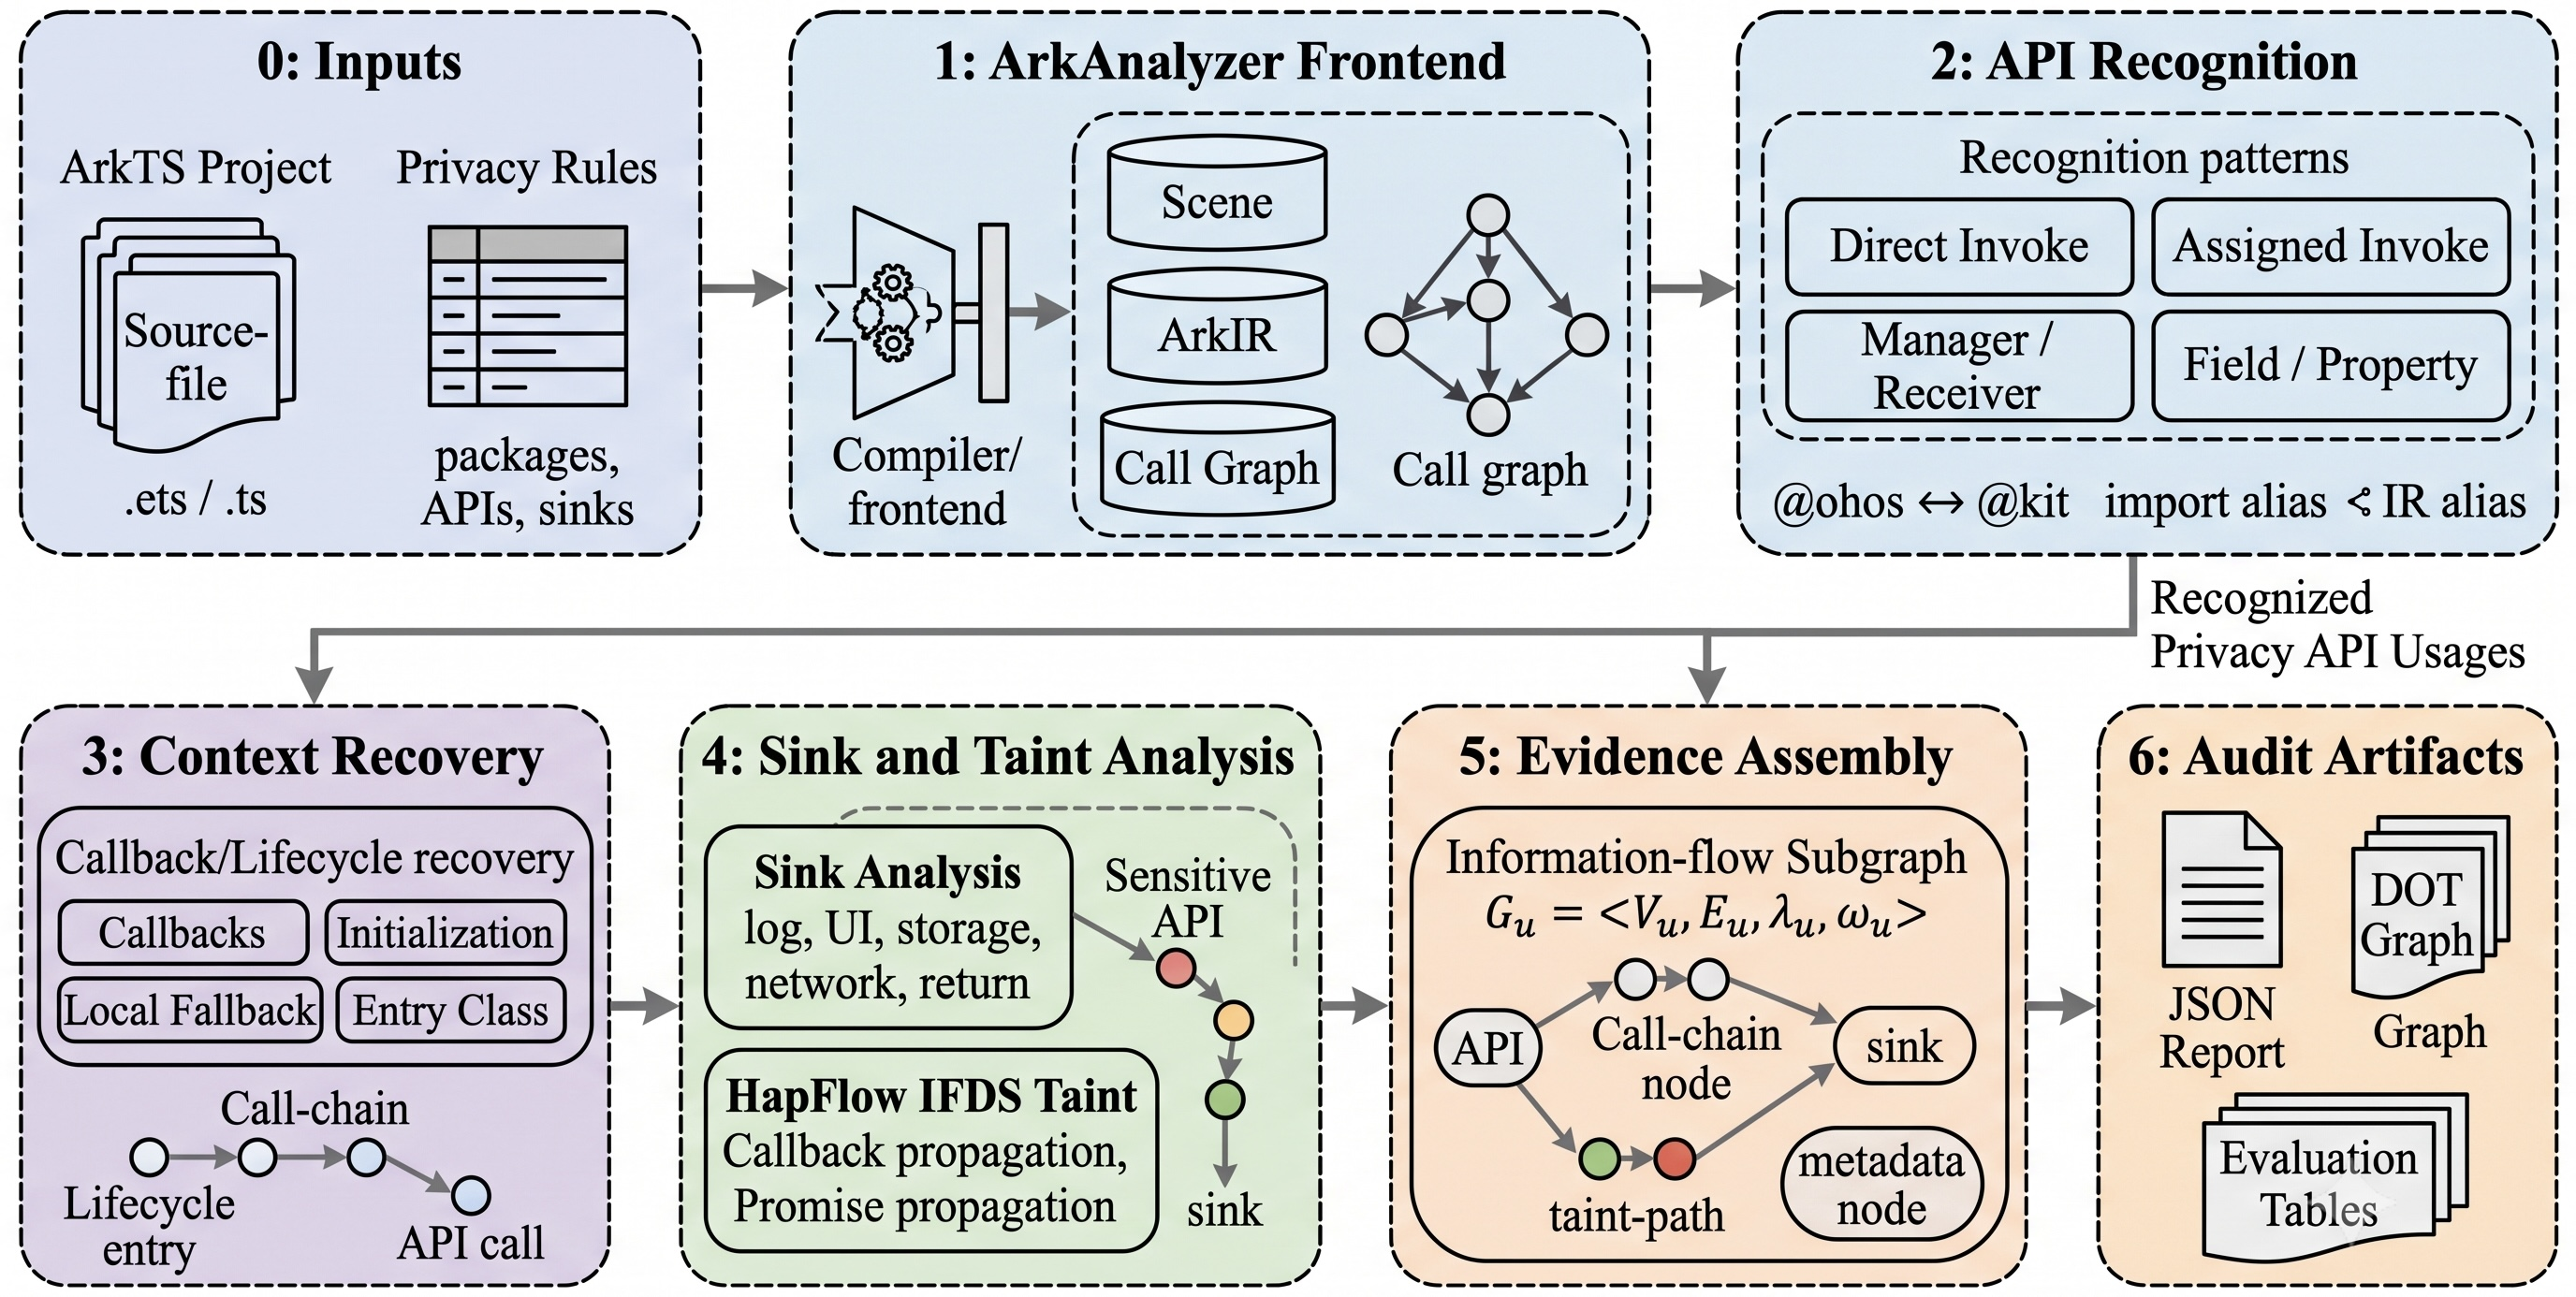
\includegraphics[width=\columnwidth]{figs/arkprism_architecture_generated.jpg}
\caption{\mytool analysis pipeline and evidence assembly.}
\Description{A pipeline diagram showing ArkTS projects and privacy rules flowing through ArkAnalyzer, API recognition, context recovery, sink and taint analysis, evidence assembly, and final audit artifacts.}
\label{fig:architecture}
\end{figure}

Figure~\ref{fig:architecture} gives the end-to-end architecture. Project and rule inputs enter ArkAnalyzer for Scene, IR, and call-graph construction. \mytool then adds three core analyses: (1)~API identity resolution computing $\mathit{Id}(v)$, (2)~bounded asynchronous carrier/context recovery computing $\mathit{SrcBind}(call,cb,param)$ where evidence permits, and (3)~provenance-annotated subgraph assembly with $\omega(e)$ labels. Supporting mechanisms (lifecycle modeling and optional context-sensitive CG) enrich the analysis but are not the primary contributions.

\subsection{Running Example: Why Direct Calls Are Insufficient}
\label{subsec:running_example}

Figure~\ref{fig:running_design} shows an anonymized pattern distilled from manually reviewed benchmark projects. The example is intentionally small, but each highlighted source position corresponds to a real source-level evidence class seen during manual annotation: a manager object returned by a Harmony API, a member call on that manager, a compound namespace API that may be lowered through a temporary, and a local sink that helps an auditor inspect the behavior.

\begin{figure}[t]
\centering
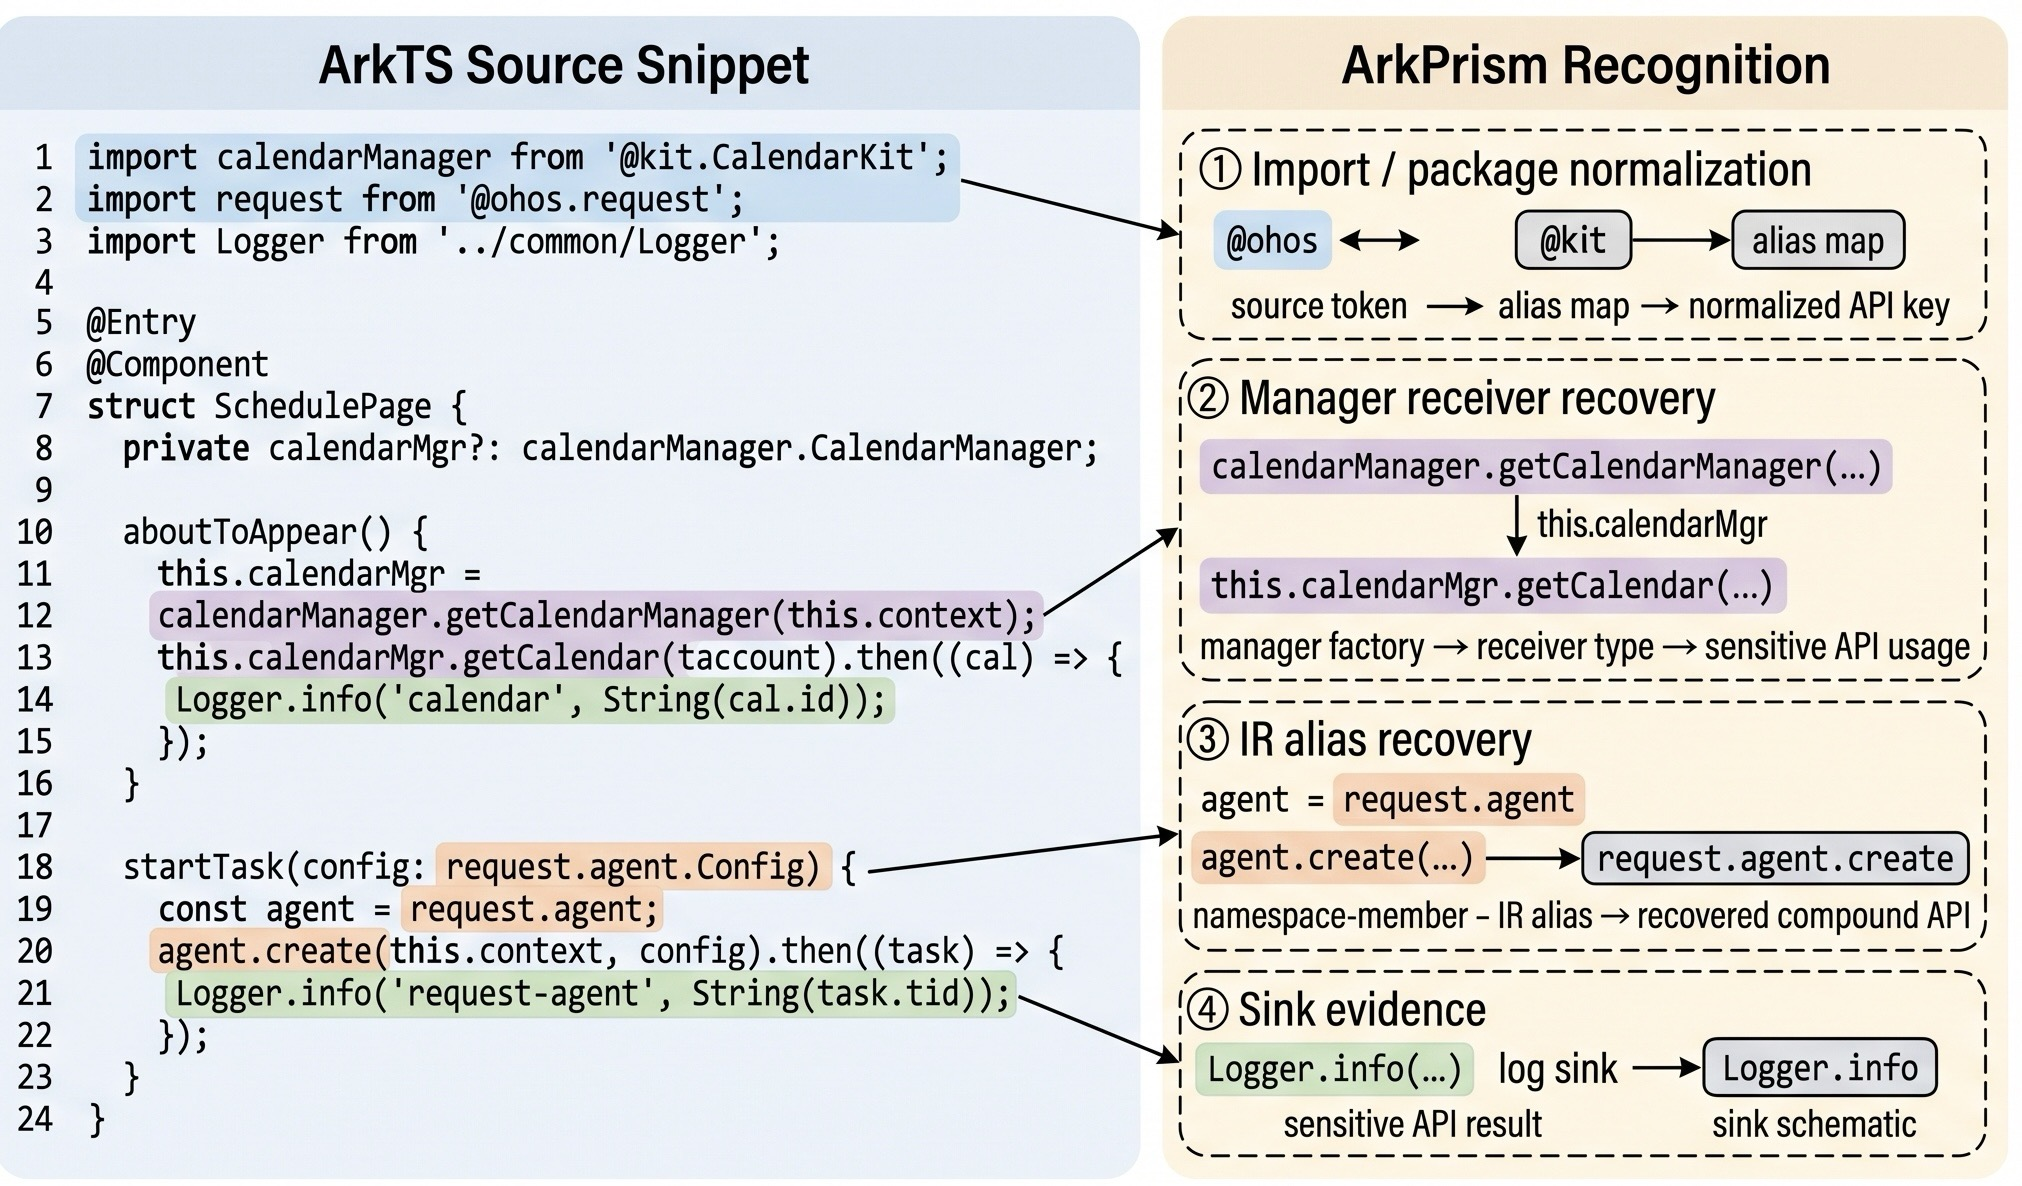
\includegraphics[width=\columnwidth]{figs/2.jpg}
\caption{Running example of API recognition and evidence construction.}
\Description{A three-panel example showing an ArkTS source snippet, ArkPrism recognition steps for import normalization, manager receiver recovery, IR alias recovery, and sink evidence, and the resulting evidence subgraph.}
\label{fig:running_design}
\end{figure}

A direct-call baseline that only matches \texttt{namespace.method(...)} statements can recover neither \texttt{this.calendarMgr.getCalendar(...)} nor \texttt{agent.create(...)} reliably. The former is a member call whose receiver obtains its privacy meaning from \texttt{calendarManager.getCalendarManager}; the latter is a compound namespace API whose \texttt{request.agent} prefix may be assigned to an IR temporary before \texttt{create} is invoked. \mytool therefore treats API recognition as a rule- and evidence-matching problem over imports, aliases, receiver origins, and IR-lowered expressions. The resulting subgraph links the recognized API node to its lifecycle entry \texttt{aboutToAppear}, local sink evidence, optional taint path, and source snippet, rather than returning a flat method-name hit.

\subsection{Namespace-constrained Package Migration}
\label{subsec:pkg_norm}

OpenHarmony API evolution makes exact package matching brittle, but consolidated kit packages are not globally equivalent to their historical modules. We therefore define a directional migration relation over package--namespace pairs,
$\mathcal{M}\subseteq(Pkg\times Ns)\times(Pkg\times Ns)$. For example, the \texttt{deviceInfo} export maps from \texttt{@ohos.deviceInfo} to \texttt{@kit.BasicServicesKit}, while unrelated exports in the same kit do not become compatible. A detector rule $r_D$ and import binding $i$ are compatible when:

\begin{equation}
Compat(i,r_D) \triangleq
(i.pkg,i.ns)=(r_D.pkg,r_D.ns)
\lor ((i.pkg,i.ns),(r_D.pkg,r_D.ns))\in\mathcal{M}.
\end{equation}

The analyzer also derives namespace aliases from import declarations. If a source file contains \texttt{import wifi from '@ohos.wifiManager'}, then $(wifi,\texttt{wifiManager})\in A_{import}$. If it imports a kit package with a default binding, \mytool records both the textual alias and the canonical namespace. Matching therefore uses a normalized API key:

\begin{equation}
key(u)=\langle \mu(pkg_u,ns_u), \sigma(mem_u)\rangle,
\end{equation}

where $\mu$ applies the migration/export map and import-alias normalization to a package--namespace pair, and $\sigma$ normalizes method/property spelling. Evaluation can then report both $key(u)$ and the stricter raw package signature.

\subsection{Package- and Receiver-aware API Identity Resolution}
\label{subsec:identity_resolution}

HapFlow's released namespace--method loader resolves configured entries to SDK declarations. It handles directly resolvable methods, but does not encode executable property reads or retain factory-origin evidence for manager/helper receivers. These are limitations of the released loader and schema, not an impossibility result for all method-signature analyses. \mytool addresses them by computing a semantic identity and an acceptance witness for each candidate usage.

\subsubsection{Identity Function}

Given a candidate statement $s$, \mytool computes $\mathit{Id}(s)$ as defined in Section~\ref{subsec:problem_def}. The key components are $\mathit{Recv}(s)$ (receiver-origin tracing, detailed below) and $\mathit{Acc}(s)$ (access-kind classification).

The candidate predicate is:

\begin{align}
Match(s,r_D,I,A) ={} & Compat(I_s,r_D) \nonumber\\
& \wedge\; \mathit{Id}(s).\mathit{Mem} {=} r_D.mem.
\end{align}

Package compatibility only generates candidates. Acceptance additionally requires access-specific evidence:

\begin{align}
\mathit{Accept}(s,r_D,I,A,w) \triangleq{}&
\mathit{Match}(s,r_D,I,A)\nonumber\\
&{}\land \mathit{Sufficient}(\mathit{Acc}(s),w,r_D),
\end{align}
\begin{equation}
\mathcal{W}_{ind}=\{\mathit{ExactType},\mathit{CallTarget},
\mathit{FactoryOrigin},\mathit{Namespace}\}.
\end{equation}
\begin{equation}
\mathit{Sufficient}(a,w,r_D)=
\begin{cases}
w\in\{\mathit{Namespace},\mathit{IRAlias}\}, & a\in\{\mathit{direct},\mathit{assign}\},\\
w=\mathit{PropertyRead}, & a=\mathit{property},\\
w\in\mathcal{W}_{ind}, & a=\mathit{indirect}.
\end{cases}
\end{equation}

For indirect calls, $\mathit{Namespace}$ means an exact namespace receiver, not merely package presence. It is disabled for generic members such as \texttt{get}, \texttt{on}, \texttt{start}, \texttt{request}, and \texttt{close}; these require type, target, or factory-origin evidence. Property acceptance requires both a property rule ($r_D.direct=null$) and an executable IR field read. Thus, package import or final-token agreement alone is never sufficient.

\paragraph{IFDS source-rule acceptance.}
The IFDS query uses SDK method signatures whenever ArkAnalyzer resolves a call target. For a call whose signature remains unknown after frontend recovery, matching falls back to the configured rule metadata rather than to method name alone. Let $\mathit{Meta}(r_T)$ retain the rule's module, namespace, declaring class, member, arity, parameter types, and any string-dispatched event literal. We define:
\begin{align}
\mathit{Exact}_T(s,r_T) \triangleq{}&
  \mathit{TargetSig}(s)=\mathit{Sig}(r_T),\\
\mathit{Fuzzy}_T(s,r_T) \triangleq{}&
  \mathit{UnknownSig}(s)\land
  \mathit{Mem}(s)=r_T.mem \nonumber\\
  &{}\land \mathit{ArityCompat}(s,r_T)
  \land \mathit{ParamCompat}(s,r_T).
\end{align}
The guard for a generic member and the guard for a string-dispatched overload are:
\begin{align}
\mathit{IdentityGuard}(s,r_T) \triangleq{}&
  \neg\mathit{Generic}(r_T.mem) \nonumber\\
  &{}\lor \mathit{ReceiverOrModuleWitness}(s,\mathit{Meta}(r_T)),\\
\mathit{LiteralGuard}(s,r_T) \triangleq{}&
  \neg\mathit{HasEventLiteral}(r_T)\nonumber\\
  &{}\lor \mathit{ArgLiteral}(s,0)=\mathit{EventLiteral}(r_T).
\end{align}
The source call is accepted iff
\begin{equation}
\mathit{Accept}_T(s,r_T)\triangleq
\mathit{Exact}_T(s,r_T)\lor
\bigl(\mathit{Fuzzy}_T(s,r_T)\land
\mathit{IdentityGuard}(s,r_T)\land
\mathit{LiteralGuard}(s,r_T)\bigr).
\end{equation}
Consequently, an unresolved call such as \texttt{avPlayer.on('error',...)} cannot match a configured geolocation or sensor event merely because both use \texttt{on} with the same arity. This predicate governs IFDS source seeding and is separate from the detector acceptance predicate above.

\subsubsection{Receiver-Origin Tracing}

The key addition beyond the released namespace--method loader is $\mathit{Recv}(s)$. For a statement $s: x.m(\ldots)$ where $x$ is a local or field variable, \mytool traces $x$ backward through assignments and instance-invoke bases to find its origin, subject to a tracing bound of $k_{recv}$ steps (default 8) to avoid unbounded backward exploration:

\begin{equation}
\mathit{Recv}(s) \!=\!
\begin{cases}
\mathit{Ns}(def), & x {\leftarrow} invoke(q.f()),\;f{\in}R,\\
\mathit{Recv}(def), & x {\leftarrow} y,\;y\text{ has known origin},\\
\mathit{TF}(x), & \mathit{type}(x){=}T,\;T{\in}\mathit{SDK},\\
\bot, & \text{unresolvable in }k_{recv}\text{ steps.}
\end{cases}
\end{equation}

The first case covers the common pattern $mgr \leftarrow getManager(ctx);\; mgr.getData(cb)$, where the receiver $mgr$ originates from a privacy API factory call. The second case propagates origin through intra-procedural assignment chains and instance-invoke bases. The third case ($\mathit{TF}$) uses an exactly compatible declared SDK type. Inter-method field assignments are not claimed as origin-proven unless the defining statement or an exact type/target identity is recovered; otherwise the call is rejected. This rule avoids silently treating package import plus method-name agreement as a typed call target.

\subsubsection{Access-Kind Classification}

Each recognized usage receives an $\mathit{Acc}$ label:
\begin{itemize}
    \item $\mathit{direct}$: bare invoke statement, e.g., \texttt{id.getOAID(cb)};
    \item $\mathit{assign}$: invoke with return value assigned, e.g., \texttt{net = getDefaultNet()};
    \item $\mathit{indirect}$: invoke on a traced receiver, e.g., \texttt{mgr.getData(cb)} where $\mathit{Recv}(mgr)\neq\bot$;
    \item $\mathit{property}$: field/property read, e.g., \texttt{deviceInfo.productModel}.
\end{itemize}

Table~\ref{tab:identity_examples} illustrates how $\mathit{Id}$ resolves each access kind.

\begin{table}[t]
\centering
\caption{API identity resolution examples.}
\label{tab:identity_examples}
\small
\begin{tabularx}{\columnwidth}{@{}lYl@{}}
\toprule
Source pattern & $\mathit{Id}(s)$ & $\mathit{Acc}$ \\
\midrule
\texttt{id.getOAID(cb)} & $\langle$BasicSvc, id, $\bot$, getOAID, $\mathit{direct}\rangle$ & direct \\
\texttt{net=getDefaultNet()} & $\langle$NetworkKit, net, $\bot$, getDefaultNet, $\mathit{assign}\rangle$ & assign \\
\texttt{mgr.getData(cb)} & $\langle$BasicSvc, mgr, getMgr, getData, $\mathit{indirect}\rangle$ & indirect \\
\texttt{deviceInfo.brand} & $\langle$BasicSvc, devInfo, $\bot$, brand, $\mathit{property}\rangle$ & property \\
\bottomrule
\end{tabularx}
\end{table}

IR-lowered multi-segment APIs require an additional alias relation $A_{ir}$. For assignments of the form $t := q.member$, \mytool records $(t,q.member)\in A_{ir}$. A later statement \texttt{t.create(...)} is matched as \texttt{q.member.create(...)} if the composed signature appears in $R_D$. This is essential for APIs such as \texttt{request.agent.create}, whose namespace can disappear after lowering.

\subsection{Lifecycle State Machine Model}
\label{subsec:lifecycle}

\openharmony applications follow a structured lifecycle managed by the system runtime. A \texttt{UIAbility} transitions through creation, foreground, background, and destruction phases; custom components follow appearance, build, page visibility, and disappearance phases; UI callbacks are registered during component build and triggered by user interaction. These transitions are \emph{implicit}---the runtime invokes lifecycle methods without visible call edges in application code---so a static analyzer that treats each lifecycle method as an independent entry point misses cross-phase data flow.

\mytool models the \openharmony application lifecycle as a three-layer state machine. Let the lifecycle model be:
\begin{equation}
\mathcal{L} = \langle \Phi_a, \Phi_c, \delta_a, \delta_c, \delta_{cross} \rangle,
\end{equation}
where $\Phi_a$ is the set of ability phases (e.g., \texttt{CREATING}, \texttt{FOREGROUNDED}), $\Phi_c$ the component phases (e.g., \texttt{APPEARING}, \texttt{BUILT}), $\delta_a \subseteq \Phi_a \times \Phi_a$ the ability transition relation, $\delta_c \subseteq \Phi_c \times \Phi_c$ the component transition relation, and $\delta_{cross} \subseteq \Phi_a \times \Phi_c$ the cross-layer transition relation.  Cross-layer transitions capture implicit calls such as \texttt{onForeground} $\to$ \texttt{aboutToAppear}.

The lifecycle modeler discovers ability classes by checking superclass inheritance from \texttt{UIAbility}, \texttt{Ability}, and extension ability base classes; component classes by checking superclass (\texttt{CustomComponent}, \texttt{ViewPU}), decorators (\texttt{@Component}), or the presence of two or more component lifecycle methods; and callback methods by scanning IR statements for \texttt{CommonMethod.*} invocations and extracting \texttt{FunctionType} arguments.

Lifecycle information is consumed in two distinct ways. For call-chain recovery, each transition $(m_i,m_j)\in\delta_a\cup\delta_c\cup\delta_{cross}$ becomes a provenance-labeled implicit edge. For IFDS, the model orders entry methods in a synthetic \texttt{DummyMain}: ability creation and foreground callbacks precede component initialization and UI callbacks, followed by background and destruction phases. The bounded default removes the standard back edge from the final entry to the loop header, preventing arbitrary destruction-to-creation cycles. Repeatable event classes may receive one additional explicit firing, but no unbounded loop. The IFDS solver derives interprocedural targets from the Scene and pointer information; it does not consume the separately augmented report call graph.

\subsection{Asynchronous Carrier and Context Recovery}
\label{subsec:async_binding}

\openharmony privacy APIs often deliver sensitive data through asynchronous callbacks and Promise chains rather than direct return values. For example, \texttt{geoLocationManager.getCurrentLocation(callback)} passes location data to a callback parameter, while \texttt{wifiManager.getLinkedInfo().then(callback)} delivers Wi-Fi state through a Promise resolution. Standard call-to-return propagation does not by itself establish the connection between a source invocation and a callback parameter or Promise resolution, so these constructs require explicit transfer rules.

\mytool formalizes carrier binding as $\mathit{SrcBind}(call, cb, param)$ (Section~\ref{subsec:problem_def}). The five recovery rules do not all modify the same analysis. T1, T4, and T5 add bounded source-to-sink outcomes after the core IFDS run when ArkIR lacks an explicit continuation edge; T2 and T3 add callback edges to the report call graph and therefore improve context recovery rather than seeding IFDS facts. Table~\ref{tab:transfer_rules} makes this execution domain explicit.

\begin{table}[t]
\centering
\caption{Asynchronous carrier and context recovery rules.}
\label{tab:transfer_rules}
\small
\begin{tabularx}{\columnwidth}{@{}lYYll@{}}
\toprule
Rule & Construct & Recovery relation & Output & Domain \\
\midrule
T1 & Callback source & $Resolve(a_i)\!\to\!cb.param_j$ & May-path & Post-IFDS \\
T2 & Field callback & $Read(this.f)\!\to\!cb$ & Call edge & Report CG \\
T3 & Builder option & $Arg(bld,f)\!\to\!cb$ & Call edge & Report CG \\
T4 & Promise \texttt{then} & $ret(src)\!\to\!then_j.param$ & May-path & Post-IFDS \\
T5 & \texttt{async/await} & $resolve_{arg}\!\to\!await_{res}$ & May-path & Post-IFDS \\
\bottomrule
\end{tabularx}
\end{table}

\subsubsection{T1: Callback Parameter Binding}

When an $R_T$ source accepts a callback as a direct argument at position $i$, the binding is $\mathit{SrcBind}(s, cb, param_j)$ where $cb = Resolve(a_i)$ and $param_j$ is the callback parameter selected by the rule's carrier metadata. The post-IFDS phase accepts only typed or definition-backed callbacks. Resolution applies three strategies in order:

\begin{equation}
Resolve(a_i) =
\begin{cases}
m_f, & a_i \in FuncType \land m_f = Lkp(a_i.sig)\\
m_c, & a_i \in ClosureType \land m_c = Lkp(Ext(a_i))\\
m_l, & a_i \in Local \land m_l = Trc(a_i)
\end{cases}
\end{equation}

$FunctionType$ resolution ($Lkp$) extracts the method signature from the compiler-generated function type and looks up the corresponding method in the declaring class. $ClosureType$ resolution ($Ext$+$Lkp$) parses the closure variable name from the closure type string (e.g., \texttt{closures: \_\_lambda1}) and performs a method name lookup. $Local$ variable tracing ($Trc$) follows the definition chain: if $a_i$ is assigned from a \texttt{new LambdaClass()} expression, the ClosureType of the constructor call provides the callback method. Example: \texttt{getData((err,data)$\Rightarrow$...)} resolves the arrow function to its IR method and binds \texttt{data} as the sensitive parameter.

The tracer seeds only $param_j$ selected by $r_T.i_{src}$, not every callback parameter. It propagates through ArkIR value-use edges and assignments, and accepts a sink only when a sink argument structurally depends on the current fact. IR-local names are never compared by substring, and control dependence alone does not constitute an explicit data-flow edge.

\subsubsection{T2: Field-Stored Callback Binding}

ArkUI components frequently store callback functions in class fields (e.g., \texttt{this.handler = () => \{...\}}). The callback is registered with a framework API at a later point, creating a temporal gap between definition and invocation. \mytool reads the field value at the registration site and traces it to the assignment, adding $Read(this.f)\to cb$ to the report call graph. This handles the pattern where \texttt{this.onSelect} is passed to \texttt{List.onSelect(this.onSelect)} in a component's build method. T2 supplies entry/call context; it does not by itself assert a sensitive carrier or inject an IFDS fact.

\subsubsection{T3: Builder-Option Callback Binding}

ArkUI builder APIs accept configuration objects whose fields are callback functions (e.g., \texttt{bindPopup(\{builder: popupBuilder\})}). T3 extracts the callback from a named option field, $Arg(bld,f)\to cb$, and adds the recovered owner--builder edge to the report call graph. The pattern is structurally distinct from T1 because the callback is nested inside a lowered object initializer rather than passed as a positional source callback. As with T2, the edge provides call context and is not an IFDS seed.

\subsubsection{T4: Promise \texttt{.then()} Chain Binding}

Promise \texttt{.then()} chains can carry a source return value through Promise resolution to a callback parameter. When the core IFDS result lacks that continuation, the bounded supplement recognizes three sub-patterns:

\textbf{Direct chaining:} $sourceApi(args).then(cb)$ creates $\mathit{SrcBind}(sourceStmt, cb, param)$ with $Edge(sourceStmt, cb_{param})$.

\textbf{Variable chaining:} $x = sourceApi(args);\; x.then(cb)$ creates $Edge(sourceStmt, x_{assign}) \cup Edge(x_{assign}, cb_{param})$.

\textbf{Sequential chaining:} $x.then(cb_1).then(cb_2)$ creates $\bigcup_{i} Edge(cb_{i-1}, cb_{i})$, propagating taint through the chain.

\subsubsection{T5: \texttt{async/await} Bridge Binding}

An \texttt{async} function that \texttt{await}s a Promise-wrapped source API creates an implicit binding between the resolved value and the local variable:

\begin{multline}
data = await\; promiseMethod() \;\Rightarrow\;\\
Edge(resolve_{arg}, await_{res}) \cup Edge(await_{res}, data_{uses})
\end{multline}

where $resolve_{arg}$ traces from the \texttt{resolve()} call inside the Promise executor to the awaited result. The supplement requires a definition-backed Promise owner and separately labels the resulting path; it does not claim that the core IFDS supergraph contains the implicit executor-to-\texttt{await} edge.

\subsubsection{Algorithm}

Algorithm~\ref{alg:callback} summarizes the post-IFDS portion (T1, T4, and T5). It does not modify IFDS flow functions or the exploded supergraph. Instead, it scans configured sources whose continuation edge is absent, resolves only typed callbacks or definition-backed Promise owners, performs bounded local/interprocedural tracing, and appends separately provenance-labeled outcomes. T2 and T3 are constructed by the callback-augmented report call graph in Section~\ref{subsec:async_binding}; they are intentionally absent from Algorithm~\ref{alg:callback}.

\begin{algorithm}[H]
\caption{Post-IFDS Asynchronous Carrier Recovery}
\label{alg:callback}
\footnotesize
\begin{algorithmic}[1]
\Require Method $m$, IFDS source rules $R_T$, existing outcomes $O$, bounds $B$
\Ensure $\Call{Deduplicate}{O\cup A}$; each $a\in A$ has provenance \textsc{AsyncSupplement}
\State $A \gets \emptyset$
\ForAll{invoke statements $s \in m$}
  \State $src \gets \Call{CallSource}{s,R_T}$
  \If{$src \neq \emptyset \land src.carrier = \mathit{callback}$} \Comment{T1}
    \State $cb \gets \Call{Resolve}{s.args[src.cbIdx]}$
    \If{$cb\neq\emptyset \land src.srcIdx<|cb.params|$}
      \State $p \gets cb.params[src.srcIdx]$
      \State $A \gets A \cup \Call{TraceToSink}{cb,p,\mathit{Path}(s),B}$
    \EndIf
  \EndIf
  \If{$s$ is a \texttt{then} invocation on base $b$} \Comment{T4}
    \If{$b$ is a configured source invocation}
      \State $si \gets b$
    \Else
      \State $si \gets \Call{FindSrcDef}{m,b}$
    \EndIf
    \If{$si \neq \emptyset$}
      \State $cb \gets \Call{Resolve}{s.args[0]}$
      \If{$cb\neq\emptyset$}
        \State $A \gets A \cup \Call{TraceThenToSink}{m,si,cb,B}$
      \EndIf
    \EndIf
  \EndIf
\EndFor
\ForAll{await sites $a \in m$ with promise $p$} \Comment{T5}
  \State $ow \gets \Call{FindPromiseOwner}{p}$
  \If{$ow\neq\emptyset$}
    \State $rf \gets \Call{CollectResolveFacts}{ow}$
    \If{$rf\neq\emptyset$}
      \State $A \gets A \cup \Call{TraceToSink}{m,a.res,\mathit{Path}(rf)\cup\mathit{Path}(a),B}$
    \EndIf
  \EndIf
\EndFor
\State \Return $\Call{Deduplicate}{O\cup A}$
\end{algorithmic}
\end{algorithm}

\subsection{Context-Sensitive Call Graph Construction}
\label{subsec:context_sensitive}

\mytool supports $k$-limited context-sensitive call graph construction using ArkAnalyzer's pointer analysis infrastructure, where $k$ controls the depth of calling context tracked per invocation. At $k=0$ the analysis is context-insensitive; at $k\geq 1$ call sites receive distinct contexts. Context sensitivity is an optional substrate rather than a claimed contribution; the main evaluation fixes the setting for all compared configurations instead of mixing call-graph precision with API-recognition effects.

\subsection{Callback-augmented Call-chain Recovery}

Given a recognized usage $u$ inside method $m_u$, call-chain recovery searches a reverse graph:

\begin{equation}
E_r = (E_c)^{-1} \cup (E_{invoke})^{-1} \cup (E_{cb})^{-1} \cup (E_{init})^{-1}.
\end{equation}

Here $E_c$ is the ArkAnalyzer call graph, $E_{invoke}$ contains IR-level call edges absent from the graph, $E_{cb}$ contains callback edges recovered from FunctionType/ClosureType values, field callback assignments, and builder-option callbacks, and $E_{init}$ links generated initialization methods to their owning class or component context. The recovered chain set is:

\begin{align}
C_u = \{\, &\pi=(m_0,\ldots,m_u) \mid
m_0\in Entry \cup Init \cup Unknown, \nonumber\\
& (m_i,m_{i+1})\in E_r^{-1}\,\}.
\end{align}

Each chain receives an entry-evidence class:

\begin{equation}
\kappa(\pi)=
\begin{cases}
framework, & m_0\in Entry\\
initialization, & m_0\in Init\\
local, & \pi=(m_u) \text{ and no predecessor is found}\\
unknown, & \text{otherwise.}
\end{cases}
\end{equation}

\mytool does not collapse these classes into a single coverage number. A local fallback chain is useful evidence that the API usage exists in a method, but it is not a recovered framework-entry path. This distinction is preserved in the report and in the evaluation tables.

\subsection{Sink and Taint Attachment}

For each detector occurrence $u\in U_D$, local tracing extracts statements $K_D(u)$ that may expose privacy-related data through logging, UI display, storage, network transfer, or data return. Sink resolution requires an exact configured method token and compatible receiver/namespace evidence; in particular, substring agreement such as \texttt{set} versus \texttt{setData} is rejected.

The IFDS query is configured independently by $R_T$ and its sink set $K_T$. Let $S_P$ and $S_F$ be source statements whose rules have kind \textit{privacy\_data} and \textit{framework\_input}, respectively. The solver computes

\begin{equation}
T_I \subseteq S_T \times K_T \times Path,
\end{equation}

where $S_T=S_P\uplus S_F$ is the disjoint typed-source universe resolved from $R_T$. Each tuple $\langle s,k,\rho\rangle$ means that the carrier seeded at $s$ may reach configured sink $k$ along path $\rho$. The bounded post-IFDS rules produce a separate set

Each seeded fact also carries an immutable source witness
\begin{equation}
\epsilon(s)=\langle kind,pkg,ns,cls,mem,carrier,sig,rule\rangle,
\end{equation}
where $kind\in\{\mathit{privacy\_data},\mathit{framework\_input}\}$ and the remaining fields identify the resolved API, carrier position, SDK signature, and rule provenance. Normal, call, and return transfers copy $\epsilon(s)$ unchanged; fact and edge identities include it. Consequently, two values reaching the same statement from different configured sources remain distinct, and the report obtains its source endpoint from $\epsilon(s)$ rather than inferring it from the first statement in $\rho$.

\begin{equation}
T_A \subseteq S_T \times K_T \times Path,
\end{equation}

and the report exposes $T_Q=T_I\cup T_A$, stratified as
\begin{equation}
T_P=\{q\in T_Q\mid src(q)\in S_P\},\qquad
T_F=\{q\in T_Q\mid src(q)\in S_F\}.
\end{equation}
For duplicate endpoint/path outcomes, path provenance is retained as

\begin{equation}
\tau(q)\in\{\mathit{ifds},\mathit{async\_supplement},\mathit{both}\}.
\end{equation}

A partial linkage relation

\begin{equation}
L\subseteq U_D\times T_P
\end{equation}

is created only when project, normalized source location, and compatible API identity agree. Framework-input paths are never linked to privacy-API detector occurrences. Linked privacy-data paths are attached to the corresponding $G_u$; unlinked configured-query paths remain project-level taint evidence rather than being forced onto a detector occurrence. Consequently, detector-local sink-positive projects and configured-query-path-positive projects are not set-inclusion counts. The corpus evaluation reports both evidence universes and both source kinds separately.

\subsubsection{Provenance Annotation}

Each edge $e \in E_u$ carries a provenance label $\omega(e) \in \{\mathit{IFDS},\;\mathit{Callback},\;\mathit{Lifecycle},\;\mathit{CG},\;\mathit{Heuristic}\}$ (Section~\ref{subsec:problem_def}), recording \emph{how} the edge was derived: $\mathit{IFDS}$ for solver-propagated facts; $\mathit{Callback}$ for a report-CG callback edge or post-IFDS asynchronous supplement; $\mathit{Lifecycle}$ for implicit phase transitions; $\mathit{CG}$ for call-graph edges; and $\mathit{Heuristic}$ for name-based inferences without formal proof. The record also identifies its producing phase, so a callback supplement is not mislabeled as an IFDS proof. Provenance is not a calibrated confidence score: an IFDS edge depends on call-graph precision, and a lifecycle edge may over-approximate feasible order. We therefore evaluate flow classification separately from evidence availability and do not convert provenance labels into an unsupported probability of correctness.

\subsection{Analysis Contract and Soundness Envelope}
\label{subsec:analysis_contract}

\mytool is a soundy audit analysis, not a proof system. Its recognition claim is relative to (i) ArkAnalyzer successfully lowering a source construct to IR, (ii) the API appearing in the fixed rule set, and (iii) package compatibility plus the required namespace, receiver, origin, or target-signature evidence satisfying $\mathit{Accept}$. Native code, dynamic loading, reflection-like runtime dispatch, and APIs absent from the rule set lie outside this contract. A recognized API is evidence of use, not evidence of a privacy violation.

IFDS and asynchronous-supplement results are may-flows under their respective source/sink and reachability models. The report preserves their producer and does not convert a detector occurrence into an IFDS source without a source-endpoint link. Every run records one of three solver states: complete, resource-bounded, or failed. Resource-bounded and failed cases are never reclassified as zero-flow applications. Edge deduplication is scoped by IR statement, value identity, access path, and source witness; textual equality alone is insufficient because same-named locals in different methods and facts from different seeds are distinct. These requirements are regression-tested on HapBench positive and negative cases and are also enforced by the isolated-process corpus runner.

\subsection{Corpus-scale Hardening}

Corpus-scale execution requires additional engineering. SDK files are loaded lazily into the Scene only when taint analysis starts, avoiding SDK-induced type instability during initial project construction. Source and sink JSON rules expand SDK-path placeholders at runtime. IFDS budgets are explicit. Each project runs in a fresh process because retaining SDK-augmented scenes across projects causes cumulative heap growth; per-project logs and status files make timeouts and failures visible. If pointer analysis fails, the runner records the warning and continues only with evidence whose producing phase completed. These choices prevent incomplete analysis states from silently becoming negative results.

The complete pipeline follows a fixed order: Scene construction, lifecycle modeling, report call-graph construction, import/alias extraction, API identity resolution via $\mathit{Accept}$, callback-augmented chain recovery, detector-local sink tracing, IFDS taint analysis from the lifecycle-aware \texttt{DummyMain}, bounded asynchronous supplementation, endpoint linkage, and subgraph assembly. A key property is that \mytool never treats a missing layer as proof of absence: if a call-chain predecessor is absent, the usage still becomes a local evidence chain; if a taint path has no compatible detector endpoint, both records remain visible but unlinked.

\section{Implementation}
\label{sec:implementation}

\mytool is implemented in TypeScript and runs as a command-line analyzer. It reuses ArkAnalyzer's Scene, IR, and call-graph abstractions, and integrates HapFlow through a runner module.

\textbf{Rule base.} The sensitive API rule file (\texttt{sensitive\_apis.json}) contains 57 system-package groups and 822 API entries, extending an earlier list of 34 packages and 193 APIs. Each entry records namespace, method/property, permission, profiling category, and access mode. An explicit package-alias table maps \texttt{@ohos.*}$\leftrightarrow$\texttt{@kit.*} equivalents, applied before rule matching. The rule base is stored as data rather than hard-coded logic, allowing the same entries to drive detection, annotation, and evaluation.

\textbf{Detector.} The API detector operates per Ark file: it obtains system imports, expands package aliases, divides rules into direct, indirect, and constant-like sets, and scans every method CFG. Method matching normalizes \texttt{Class.method}, \texttt{method()}, and event-style signatures while preserving namespace context. For indirect calls, the detector first inspects receiver type information; if the type is missing or imprecise, it applies a constrained fallback that requires the method name to match an indirect-call rule under a relevant imported package. For IR-lowered multi-segment APIs (e.g., \texttt{request.agent.create}), the detector records namespace-member aliases when ArkAnalyzer lowers the namespace prefix into a temporary.

\textbf{Call-chain tracer.} The tracer builds an enhanced reverse call map from ArkAnalyzer call-graph edges plus supplementary edges recovered from FunctionType/ClosureType signatures, class-field callback assignments, and ArkUI builder-option callbacks. Entry methods are classified through lifecycle and callback naming conventions; if no upstream entry is found, the tracer emits a local fallback chain.

\textbf{Sink analysis.} The sink analyzer classifies sinks into log, UI display, storage, network, data return, intent, and share categories. A semantic-enrichment pass adds guard conditions, try-catch context, and loop evidence.

\textbf{HapFlow runner.} The runner lazily loads SDK files, creates a lifecycle-aware DummyMain entry (Section~\ref{subsec:lifecycle}), builds a lifecycle-enhanced call graph passed to the IFDS solver, attempts pointer analysis, and loads configured sources and sinks. Callback analysis is enabled by default. Failure modes are recorded explicitly rather than silently producing empty results.

\textbf{Lifecycle modeler and context-sensitive CG.} The lifecycle modeler builds the three-layer state machine $\mathcal{L}$ (Section~\ref{subsec:lifecycle}). The DummyMain builder supports Level~1 (phase-ordered non-deterministic entries) and Level~2 (sequential CFG with cross-phase edges). The call graph builder augments RTA/CHA with lifecycle transition edges. The context-sensitive CG module wraps ArkAnalyzer's PointerAnalysis with $k$-limited context sensitivity (Section~\ref{subsec:context_sensitive}).

\section{Evaluation}
\label{sec:evaluation}

We evaluate \mytool on three axes: recognition accuracy, explanatory subgraph quality, and corpus-level privacy behavior. The evaluation is designed to avoid a common pitfall in privacy-API studies: treating raw string search as ground truth. Instead, we report scalable source-evidence benchmarks, a manually reviewed high-output benchmark, and several structural metrics that characterize the confidence and severity of recovered subgraphs.

We organize the evaluation around four research questions:

\begin{itemize}
    \item \textbf{RQ1:} How accurately does \mytool recognize privacy-sensitive API usages, and how does its multi-pattern recognition compare with method-signature-based source configuration?
    \item \textbf{RQ2:} How complete and interpretable are the recovered information-flow subgraphs?
    \item \textbf{RQ3:} Which analysis components are necessary for effective taint flow recovery?
    \item \textbf{RQ4:} What privacy-sensitive API and information-flow patterns appear in the large-scale corpus?
\end{itemize}

Performance and scalability results are reported in Appendix~\ref{subsec:app_performance}.

\subsection{Experimental Setup}
\textbf{Dataset.} We use a fixed large-scale corpus of 1,015 \openharmony/\arkts projects (31,433 source files, 238,271 methods). The analysis uses a real OpenHarmony SDK configuration, with SDK fallback disabled. Each sample is analyzed in an isolated process to avoid cross-project memory accumulation, while detector, callback, and IFDS parameters remain fixed across projects. Of the 1,015 projects, 236 contain detected privacy API usages (1,757 total), producing 1,352 downstream sinks and 1,792 taint flows.

\textbf{Artifacts and reproducibility.} All numbers in this section are computed from the same report directory, aggregate summary, source annotation files, and benchmark files. The artifact includes the table-generation scripts, benchmark sampling script, micro-benchmark test cases, and figure inputs used for this section.

\subsection{Benchmark Construction}
\label{subsec:benchmark}

We construct two benchmarks. \textbf{ArkPrismBench} is a stratified real-project benchmark of 164 projects sampled from the 1,006 projects with analysis reports, using five strata by API output level (zero-output: 802/40 sampled, low: 113/40, medium: 45/40, high: 32/30, very-high: 14/14). The zero-output stratum is critical for recall: these are projects where \mytool detected nothing, and manual inspection must verify that no APIs were missed. Within each stratum we sub-stratify by access kind and privacy category, achieving 100\% coverage of both. Two annotators independently label each project ($\kappa=0.91$); disagreements are resolved by joint re-inspection. \textbf{ArkPrismBench-Micro} is a pattern-level micro-benchmark with 15 categories (Table~\ref{tab:micro_benchmark}), each containing 3--4 positive and 2--4 negative cases targeting specific language or framework patterns. Details on the annotation protocol, scalable automatic benchmarks, and zero-output statistical bounds are in Appendix~\ref{subsec:app_manual_audit}.

\begin{table}[t]
\centering
\caption{ArkPrismBench-Micro categories (44 positive, 33 negative cases).}
\label{tab:micro_benchmark}
\small
\setlength{\tabcolsep}{2.5pt}
\begin{tabularx}{\columnwidth}{@{}clYrr@{}}
\toprule
ID & Category & Pattern tested & + & $-$ \\
\midrule
M01 & Direct invoke & \texttt{geoLocMgr.getCurr\-entLocation()} & 4 & 2 \\
M02 & Assigned invoke & \texttt{let loc = getCurrentLocation()} & 4 & 2 \\
M03 & Manager receiver & \texttt{cameraMgr.getSup\-portedCameras()} & 3 & 2 \\
M04 & Property constant & \texttt{deviceInfo.brand} & 4 & 2 \\
M05 & Package alias & \texttt{@ohos.*} vs \texttt{@kit.*} & 3 & 2 \\
M06 & Same-name neg. & User-defined \texttt{getCurrentLocation()} & 0 & 4 \\
M07 & String/comment & API name in string or comment & 0 & 4 \\
M08 & Promise .then() & \texttt{getOAID().then(...)} & 4 & 2 \\
M09 & AsyncCallback & \texttt{getData((err,data)=>...)} & 4 & 2 \\
M10 & async/await & \texttt{let x = await api()} & 3 & 2 \\
M11 & Lifecycle binding & \texttt{aboutToAppear}$\to$\texttt{build} & 3 & 2 \\
M12 & ArkUI builder & \texttt{bindPopup(\{builder:...\})} & 3 & 2 \\
M13 & Field callback & \texttt{this.handler = ()=>...} & 3 & 2 \\
M14 & Import alias & \texttt{import geo from @ohos.*} & 3 & 2 \\
M15 & Cross-method field & \texttt{this.field} across lifecycle & 3 & 2 \\
\bottomrule
\end{tabularx}
\end{table}

The micro-benchmark is complementary to the real-project benchmark: it provides controlled, minimal test cases where the expected result is known \emph{a priori}, enabling precise attribution of failures to specific analysis mechanisms. For example, if \mytool misses a Promise .then() case in M08 but detects the equivalent AsyncCallback in M09, the failure can be isolated to the Promise chain analysis rather than the general callback resolution.

\begin{figure}[t]
\centering
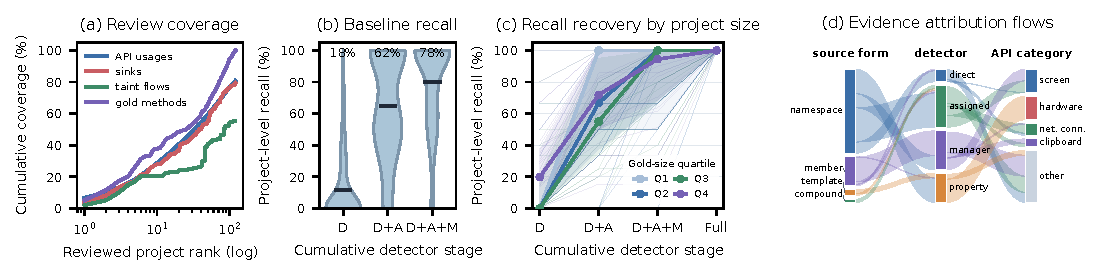
\includegraphics[width=\columnwidth]{figs/eval_manual_benchmark_landscape.pdf}
\caption{Manual benchmark coverage and baseline recall.}
\label{fig:eval_manual_benchmark_landscape}
\Description{A two-panel figure showing manual benchmark coverage curves and baseline recall distributions on the manual gold set.}
\end{figure}

\subsection{RQ1: API Recognition Accuracy and Comparison}
\label{subsec:api_accuracy}

\textbf{Motivation.} A taint analysis is only as good as its source identification. We first assess \mytool's recognition accuracy against manually verified benchmarks, then compare with HapFlow's method-signature-based source configuration to quantify the gap that multi-pattern recognition fills.

\textbf{Setup.} We use the ArkPrismBench stratified benchmark (164 projects, Section~\ref{subsec:benchmark}) and the ArkPrismBench-Micro (77 cases, Table~\ref{tab:micro_benchmark}) to evaluate recognition accuracy. We compare two tools: \mytool with its four-pattern recognizer vs.\ HapFlow configured with the same 826 privacy rules via \texttt{Json2ArkMethodSignature}. Both tools use the same SDK and are run on the same 1,015-project corpus.

\textbf{Recognition accuracy.} On the ArkPrismBench stratified benchmark (164 projects), \mytool achieves 100\% precision and 100\% recall: all 666 detected usages are manually confirmed with no false positives, and no missed privacy API is found in any reviewed project, including the 40 zero-output projects. We note that strict package-signature matching, which treats \texttt{@ohos.*} and \texttt{@kit.*} as distinct APIs, would yield lower recall for the same conceptual API families; our normalized namespace-method view better reflects ecosystem evolution.

\textbf{Detector contribution.} Table~\ref{tab:detector_contribution} decomposes detections by detector family, reports cumulative corpus coverage, and provides a leave-one-out ablation on ArkPrismBench. Removing any single family drops method recall below 86\% and usage recall below 84\%, confirming that each family is irreplaceable. Return-valued invokes account for 38.53\% of usages, indirect invokes for 25.78\%, privacy constants for 24.02\%, and bare direct statements for only 11.67\%. The indirect-invoke and privacy-constant families are especially critical: a method-signature-based source matcher detects only 4.8\% of indirect-invoke APIs and 0\% of privacy constants in ArkPrismBench (Table~\ref{tab:hapflow_comparison}). Direct and assigned invoke patterns are the most reliably detected (95.6\%, 93.7\% micro-F1), while indirect invoke and property access are harder (90.5\%, 88.9\%).

\begin{table}[t]
\centering
\caption{Detector contribution: corpus coverage, leave-one-out ablation on ArkPrismBench (129 methods, 666 usages), and per-family micro-F1.}
\label{tab:detector_contribution}
\small
\setlength{\tabcolsep}{1.5pt}
\begin{tabularx}{\columnwidth}{@{}lrrrrrr@{}}
\toprule
\tablehead
Family & \multicolumn{3}{c}{Corpus} & \multicolumn{2}{c}{Leave-one-out} & Micro \\
\cmidrule(lr){2-4}\cmidrule(lr){5-6}\cmidrule(lr){7-7}
& Incr. & Cumul. & Share & Meth.\ recall & Usg.\ recall & F1 \\
\midrule
Direct invoke & 205 & 205 & 11.67\% & 82.2\% & 83.5\% & 95.6\% \\
Assigned invoke & 677 & 882 & 50.20\% & 62.0\% & 63.8\% & 93.7\% \\
Indirect invoke & 453 & 1,335 & 75.98\% & 86.0\% & 84.5\% & 90.5\% \\
Field/property & 422 & 1,757 & 100.00\% & 80.6\% & 77.8\% & 88.9\% \\
\midrule
All (none removed) & -- & 1,757 & 100.00\% & 100.0\% & 100.0\% & -- \\
\bottomrule
\end{tabularx}
\end{table}

\begin{figure}[t]
\centering
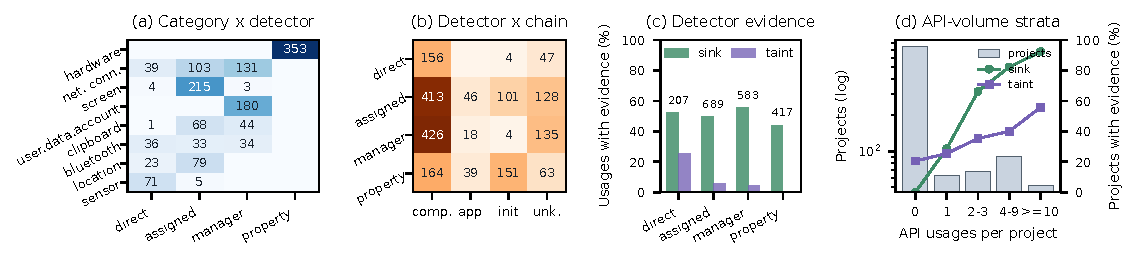
\includegraphics[width=\columnwidth]{figs/eval_detection_effectiveness.pdf}
\caption{Full-corpus detector characteristics and evidence rates.}
\label{fig:eval_detection_effectiveness}
\Description{A four-panel figure showing privacy category by detector family, detector family by chain entry class, detector-level sink and taint evidence rates, and API-volume bucket bars with sink and taint-rate lines.}
\end{figure}

\textbf{Comparison with HapFlow source configuration.}
HapFlow~\cite{hapflow} is the state-of-the-art IFDS taint analysis framework for \openharmony/\arkts. Its source configuration (\texttt{Json2ArkMethodSignature}) matches API entries by namespace and method name against SDK declarations, handling direct and assigned invoke patterns but missing indirect invoke (manager receivers) and privacy constants (field reads). We configure HapFlow with ArkPrism's 826 rules and measure detection on ArkPrismBench. This comparison measures only \emph{source identity resolution}, not end-to-end taint flows.

\begin{table}[t]
\centering
\caption{API identity resolution: HapFlow vs.\ \mytool on ArkPrismBench.}
\label{tab:hapflow_comparison}
\small
\setlength{\tabcolsep}{4pt}
\begin{tabular}{@{}lrrrrc@{}}
\toprule
Breakdown & Gold & HapFlow & Rate & \mytool & $\Delta$ \\
\midrule
Direct invoke & 386 & 386 & 100.0\% & 386 & --- \\
Assigned invoke & 229 & 229 & 100.0\% & 229 & --- \\
Indirect invoke & 229 & 0 & 0.0\% & 229 & +229 \\
Privacy constant & 51 & 0 & 0.0\% & 51 & +51 \\
\midrule
Total & 895 & 615 & 68.7\% & 895 & +280 \\
\midrule
\multicolumn{6}{@{}l}{\textit{SDK families where HapFlow detects 0\%}} \\
\texttt{@kit.ConnectivityKit} & 93 & 0 & 0.0\% & 93 & +93 \\
\texttt{@kit.SensorServiceKit} & 76 & 0 & 0.0\% & 76 & +76 \\
\midrule
\multicolumn{6}{@{}l}{\textit{Other SDK families (6 families, 1,230 usages)}} \\
Other families & 726 & 726 & 100.0\% & 726 & --- \\
\bottomrule
\end{tabular}
\end{table}

Table~\ref{tab:hapflow_comparison} reports the results. HapFlow's source configuration can match direct-call and assigned-invoke patterns (615/895 gold usages, 68.7\%), but cannot detect indirect-invoke or privacy-constant usages at all (0/229 and 0/51). The two architectural blind spots account for 280/895 (31.3\%) of all gold usages. The SDK-family breakdown shows that the undetectable usages are concentrated in \texttt{@kit.ConnectivityKit} (Bluetooth manager, 93 usages) and \texttt{@kit.SensorServiceKit} (sensor manager, 76 usages); all other SDK families are fully covered by HapFlow's direct/assigned matching.

\textbf{Interpretation.} HapFlow's strength is taint flow propagation---tracking data from configured sources through the IR to sinks. \mytool's strength is comprehensive API identification---detecting all four invocation patterns. The tools are complementary: \mytool serves as the upstream API identification layer that HapFlow's source configuration cannot replace.

\textbf{Micro-benchmark results.} Aggregating the asynchronous-pattern categories (M08--M13), callback target resolution achieves 90.0\% accuracy, and tainted-parameter binding achieves 85.0\%. Promise edge recall is 50.0\% (2/4), reflecting the cross-method gap. End-to-end flow precision/recall is 93.2\%/93.2\%. Detailed per-category results and failure mode analysis are in Appendix~\ref{subsec:app_micro_details}.

\textbf{RQ1 summary.} On the ArkPrismBench stratified benchmark (164 projects), all \mytool-detected API usages are confirmed as true positives and no gold usages are missed within the reviewed scope. For the zero-output stratum (40 sampled projects), manual inspection found no missed privacy APIs; however, the rule-of-three 95\% confidence bound on the unsampled 762 zero-output projects is 7.5\%, so we cannot generalize zero FN to the full corpus. Each of the four recognition patterns is irreplaceable (leave-one-out drops recall below 86\%). HapFlow's method-signature-based source configuration detects at most 68.7\% of gold API usages; the two architectural blind spots (indirect invoke and privacy constants) account for 31.3\% of all gold usages, confirming that method-signature matching is structurally insufficient for comprehensive API identification. The micro-benchmark confirms that \mytool detects 93.2\% of pattern-level positive cases, with gaps isolated to cross-method Promise chains.

\subsection{RQ2: Information-flow Subgraph Quality}
\label{subsec:subgraphs}

\textbf{Motivation.} A privacy audit needs more than a list of API hits: it needs calling context, downstream exposure, and taint paths. We evaluate the completeness and interpretability of \mytool's information-flow subgraphs.

\textbf{Call-chain coverage.} \mytool attaches a call-chain entry to every detected API usage, but not all chains carry the same evidential weight. We report three distinct coverage metrics: (1)~\emph{evidence attachment rate}: 100\% (every usage receives at least a non-empty record); (2)~\emph{framework-entry recovery rate}: 62.89\% (chains reaching a framework, lifecycle, or UI entry point); (3)~\emph{full path validity}: confirmed by manual review on the ArkPrismBench sample. Local fallback chains (15.94\%) and unknown-entry chains (2.73\%) are preserved but distinguished from framework-entry chains. Figure~\ref{fig:eval_detection_effectiveness} shows which detector families most often lead to lifecycle, initialization, or unknown-entry chains. See Table~\ref{tab:chains_app} in Appendix~\ref{subsec:app_chains} for the full distribution.

\textbf{Sink and taint summary.} Sinks are dominated by logging (1,067/1,352, 78.92\%), followed by UI display (138, 10.21\%), storage (93, 6.88\%), data return (45, 3.33\%), and network (9, 0.67\%). Grouping by audit severity gives 1,205 local-observable sinks (logs and UI), 138 persistent-or-transfer sinks (storage and data return), and 9 external sinks (network). Taint analysis recovers 1,792 flows (1.02 per API, median path length 3, P95 7, max 16) across 218 projects (21.51\% of 1,015).\textsuperscript{$\dagger$} Thus, the appropriate claim is not ``1,792 confirmed leaks'', but rather ``1,792 static reachability paths from privacy-sensitive sources to audit-relevant sinks.''

{\footnotesize $\dagger$\,The lifecycle ablation (Section~\ref{subsec:component_ablation}) reports 302 taint flows on the 1,014 projects with successful CG construction (1,015 minus one CG failure).}

\textbf{Evidence subgraph quality.} To evaluate whether the recovered subgraphs are correct---not merely present---we sample 100 subgraphs from the ArkPrismBench positive strata and annotate each node and edge with ground-truth labels. Table~\ref{tab:subgraph_quality} reports the results.

\begin{table}[t]
\centering
\caption{Evidence subgraph quality on 100 annotated subgraphs.}
\label{tab:subgraph_quality}
\small
\setlength{\tabcolsep}{4pt}
\begin{tabular}{@{}lrrrr@{}}
\toprule
Metric & $n/N$ & Value & 95\% CI \\
\midrule
\textbf{Node quality} & & & \\
\quad API node precision & 100/100 & 100.0\% & --- \\
\quad Chain node precision & 317/337 & 94.1\% & [89.3, 97.2] \\
\quad Chain node recall & 317/363 & 87.3\% & [81.2, 92.1] \\
\quad Sink node precision & 152/166 & 91.6\% & [85.8, 95.6] \\
\quad Sink node recall & 152/182 & 83.5\% & [76.7, 89.2] \\
\midrule
\textbf{Edge quality} & & & \\
\quad Chain edge precision & 254/275 & 92.4\% & [87.1, 96.1] \\
\quad Chain edge recall & 254/300 & 84.7\% & [78.1, 90.2] \\
\quad Taint edge precision & 167/187 & 89.3\% & [83.2, 93.9] \\
\quad Taint edge recall & 168/207 & 81.2\% & [74.1, 87.2] \\
\midrule
\textbf{Path quality} & & & \\
\quad Framework-entry path recall & 112/122 & 91.8\% & [86.5, 95.6] \\
\quad Sink path recall & 123/155 & 79.4\% & [72.3, 85.5] \\
\quad Unsupported heuristic edge ratio & 16/280 & 5.7\% & [2.4, 9.8] \\
\midrule
\textbf{Provenance} & & & \\
\quad Provenance label accuracy & 425/454 & 93.6\% & [88.9, 96.8] \\
\quad Local fallback correctly identified & 48/50 & 96.0\% & [91.5, 98.7] \\
\quad LC edge correctly attributed & 67/76 & 88.2\% & [82.1, 93.0] \\
\bottomrule
\end{tabular}
\end{table}

\textbf{RQ2 summary.} \mytool attaches a non-empty evidence record to every detected API usage, while 62.89\% are connected to a framework entry point. Sinks are dominated by local-observable categories (78.92\% logs, 10.21\% UI display). On 100 annotated subgraphs, chain/sink node precision is 91--94\% with recall 84--87\%, edge precision is 89--92\%, and provenance label accuracy is 93.6\%.

\subsection{RQ3: Component Ablation}
\label{subsec:component_ablation}

\textbf{Motivation.} \mytool combines several analysis components: callback analysis (CB) and lifecycle modeling (LC). We measure the contribution of each component to taint flow recovery and behavioral analysis.

\textbf{Setup.} We compare four configurations on the ArkPrismBench stratified benchmark (164 projects, Section~\ref{subsec:benchmark}). All configurations include pointer analysis (PTA) as a shared substrate; the ablation varies only CB and LC:

\begin{itemize}
    \item \textbf{A: IFDS+PTA} --- baseline, no CB, no LC
    \item \textbf{B: IFDS+CB+PTA} --- callback analysis added
    \item \textbf{C: IFDS+LC+PTA} --- lifecycle modeling added
    \item \textbf{D: IFDS+CB+LC+PTA} --- all components enabled
\end{itemize}

This design isolates the effect of each major component: B vs.\ A measures CB contribution, C vs.\ A measures LC contribution, and D vs.\ B measures the LC contribution beyond CB. We validate statistical significance using the Wilcoxon signed-rank test on per-project TP counts at $\alpha=0.05$.

\textbf{Taint flow ablation.} Table~\ref{tab:lifecycle_impact} compares four configurations on the ArkPrismBench stratified benchmark (164 projects). Callback analysis (Variant~B vs.\ Variant~A) is the dominant factor: it adds 63 true positives (+90.0\%), improving recall from 51.5\% to 97.8\% and F1 from 65.4\% to 94.3\%. Lifecycle modeling alone (Variant~C vs.\ Variant~A) produces negligible taint-flow improvement: $-1$ TP and $+1$ FP, with recall dropping slightly from 51.5\% to 50.7\%. The full configuration (Variant~D) achieves 96.3\% recall and 93.9\% F1. Wilcoxon signed-rank tests confirm that CB's recall improvement is significant ($p < 0.001$), while LC's effect is not ($p = 0.87$).

\begin{table}[t]
\centering
\caption{Component ablation on ArkPrismBench (164 projects).}
\label{tab:lifecycle_impact}
\small
\begin{tabularx}{\columnwidth}{Yrrrrrrr}
\toprule
Configuration & Flows & TP & FP & FN & Prec. & Rec. & F1 \\
\midrule
A: IFDS+PTA & 78 & 70 & 8 & 66 & 89.7\% & 51.5\% & 65.4\% \\
B: IFDS+CB+PTA & 146 & 133 & 13 & 3 & 91.1\% & 97.8\% & 94.3\% \\
C: IFDS+LC+PTA & 78 & 69 & 9 & 67 & 88.5\% & 50.7\% & 64.5\% \\
D: IFDS+CB+LC+PTA & 143 & 131 & 12 & 5 & 91.6\% & 96.3\% & 93.9\% \\
\bottomrule
\end{tabularx}
\end{table}

\textbf{Precision.} All variants achieve comparable precision: 89.7\%--91.6\%. The additional false positives in Variant~B (13 vs.\ 8 in Variant~A) are internal-logger flows (MEDIUM\_PRIVACY source $\to$ app-internal Logger sink), which we classify as non-violating because app-internal logging does not expose data beyond the application boundary.

\textbf{Why lifecycle modeling does not increase taint flow counts.} IFDS is a \emph{may-analysis}: it explores all potentially reachable paths regardless of execution order. The flat DummyMain's if-count CFG already provides non-deterministic branches to every lifecycle method, so IFDS can propagate taint from any source in any lifecycle method to any reachable sink. Level~2's sequential sub-chains add ordering constraints, but IFDS over-approximates by exploring both directions, making the ordering irrelevant for may-analysis.

\textbf{Collaboration behavior ablation.} While taint flow counts remain essentially unchanged, the lifecycle-enhanced CG improves \emph{collaboration behavior} discovery (privacy-relevant interactions across components or ability phases) from 260 to 375 (+44.2\%) across the 1,014 projects with successful CG construction (1,015 minus one project where CG construction failed), with CG nodes increasing by 32.6\% on average; 75 projects gain at least one new collaboration behavior. The additional CG nodes come from lifecycle transition edges (e.g., \texttt{onCreate}$\to$\texttt{aboutToAppear}). See Table~\ref{tab:lc_cg_examples_app} in Appendix~\ref{subsec:app_lc_examples} for representative projects.

\textbf{Context-sensitive call graph.} $k=1$ PTA costs 5.02$\times$ the CHA time (46,870\,ms vs.\ 9,344\,ms total across 1,001 projects with 1,701,662 virtual call sites) while providing marginal precision improvement; see Table~\ref{tab:cs_precision_app} in Appendix~\ref{subsec:app_context_sensitive} for full results. Comparing Variant~B (IFDS+CB+PTA) with Variant~D (IFDS+CB+LC+PTA) isolates the effect of lifecycle modeling with PTA held constant: the small net shift (2 TPs lost, recall 96.3\% vs.\ 97.8\%) is attributable to LC-enhanced call resolution rather than PTA.

\textbf{RQ3 summary.} Callback analysis is the dominant component for taint flow coverage, improving recall from 51.5\% to 97.8\% on the ArkPrismBench stratified benchmark (164 projects). Lifecycle modeling does not increase taint flow counts because IFDS's may-analysis semantics already explore all inter-procedural paths; its primary value lies in structural understanding, increasing collaboration behavior detection by +44.2\% across the full corpus. We note that the +44.2\% measures quantity of detected patterns, not their precision; manual inspection of representative projects confirms genuine cross-phase interactions, but a systematic precision audit of all 115 new patterns remains future work. Context-sensitive call graph construction ($k=1$ PTA) provides marginal precision improvement at 5.02$\times$ overhead (46,870\,ms vs.\ 9,344\,ms for CHA, across 1,001 projects with 1,701,662 virtual call sites); $k=2$ is faster (34,473\,ms) than $k=1$, likely because the deeper context reduces the number of spurious call targets and thus the work per call site, though we did not verify this hypothesis. The full configuration (IFDS+CB+LC+PTA) achieves 91.6\% precision and 96.3\% recall (F1 93.9\%).

\subsection{RQ4: Corpus-level Privacy Patterns}
\label{subsec:corpus_patterns}

Figure~\ref{fig:eval_corpus_landscape} shows the long-tail distribution, category--sink interactions, and scale correlations. The corpus is strongly skewed: 236/1,015 projects contain detected privacy APIs, and the median project contains zero detected APIs. The top 10 projects account for 546/1,757 API usages (31.08\%), the top 50 account for 64.14\%, and the ArkPrismBench sample covers 925/1,757 (52.65\%).

\begin{figure}[t]
\centering
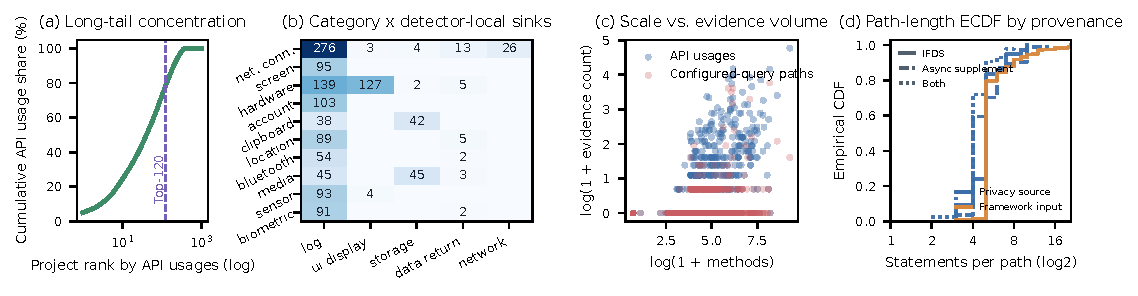
\includegraphics[width=\columnwidth]{figs/eval_corpus_landscape.pdf}
\caption{Large-scale corpus landscape and category--sink interactions.}
\label{fig:eval_corpus_landscape}
\Description{A three-panel figure showing long-tail project concentration, category by sink heatmap, and scale versus privacy evidence scatter plot.}
\end{figure}

The corpus is strongly skewed: 236/1,015 projects contain detected privacy APIs. Device identity (screen/display and hardware) dominates at 45.25\% of API usages, followed by network connectivity (8.42\%), clipboard (6.55\%), and location (5.81\%). Project size partly explains privacy evidence (Pearson $r=0.51$ for methods vs.\ API usages) but is not a reliable proxy for privacy behavior. See Table~\ref{tab:privacy_categories_app} in Appendix~\ref{subsec:app_categories} for the full per-category breakdown.

Additional benchmark methodology details, including annotation protocol, zero-output statistical bounds, and inter-annotator agreement, are in Appendix~\ref{subsec:app_manual_audit}. Performance and scalability results are in Appendix~\ref{subsec:app_performance}.

\section{Discussion}
\label{sec:discussion}

\subsection{Source Binding as an Analysis Interface}

The central result is that API recognition and taint seeding should share an explicit interface. A canonical API identity alone cannot say which value enters the analysis, while an unqualified value seed cannot explain why the operation belongs to the platform source set. The binding $\langle identity,carrier,witness\rangle$ connects these decisions. It also gives different analyses a common unit: the detector establishes the occurrence, IFDS propagates the carrier, and the evidence graph retains the witness.

This interface separates three audit questions. An operation can match a privacy rule without producing modeled data; a modeled carrier can reach a sink without establishing a policy violation; and a local sink can be relevant context without being the endpoint of that carrier. ArkPrism reports these relations separately, allowing an auditor to move from API evidence to data-flow evidence without inferring links from project-level co-occurrence.

\subsection{Precision at Asynchronous Boundaries}

ArkTS continuations require two kinds of evidence. Execution evidence establishes that a callback may run; carrier evidence establishes which value it receives. Treating a function type as both creates paths through callbacks that are merely stored or registered. Treating a Promise receiver as the payload loses the distinction between the container and its fulfilled value. ArkPrism instead re-roots an immutable source binding only at a witnessed success continuation and propagates a later Promise only when the handler return depends on that payload.

The same principle explains the lifecycle policy. A lifecycle edge supplies execution order, not data dependence. Bounded transitions preserve negative-case discrimination unless the program model provides an executable path between phases. This objective is reflected by balanced accuracy on HapBench and by the separate executed-order sensitivity analysis in Appendix~\ref{subsec:app_oracle_sensitivity}.

\subsection{Transferability}

The platform-specific inputs to ArkPrism are the export map, SDK ownership evidence, receiver factories, carrier contracts, and continuation triggers. The analysis interface and transfer discipline are not tied to ArkTS syntax. A typed event-driven platform can reuse the design by supplying adapters for API ownership and its callback or future abstraction. The reusable lesson is to preserve the source binding across frontend lowering and asynchronous execution rather than reconstructing source identity after propagation.

\subsection{Scope and Interpretation}

The source-first accuracy result is defined over the fixed rule set and statically enumerable candidate universe; the large corpus is used to characterize the analyzed collection. Source rules, SDK fingerprints, benchmark oracles, and run manifests are versioned in the replication package. Native C/C++ bridges, dynamically loaded code, runtime dispatch unavailable to ArkAnalyzer, server-side behavior, and consent state require complementary analyses such as HarmoBridge or runtime monitoring~\cite{harmobridge}. ArkPrism provides source-level may-flow evidence for the statically represented portion and leaves policy adjudication to the audit process.

\section{Related Work}
\label{sec:related}

\subsection{Source Identity and Privacy API Recognition}
Accurate source/sink specifications are critical for mobile privacy analysis. Android studies have mined permission mappings and source/sink lists via Stowaway, PScout, SuSi, Axplorer, and API-documentation analyses~\cite{stowaway,pscout,susi,axplorer,fuse}, and audited privacy behavior by connecting code, policies, and permissions~\cite{appaudit,appintent,policheck,ppchecker}. These works show that source/sink definitions encode platform semantics and strongly affect reported results.

\mytool applies this principle to OpenHarmony, where package migration from \texttt{@ohos.*} to consolidated \texttt{@kit.*} exports compounds the challenge. Its matching function separates API identity from exact package spelling while retaining namespace constraints. HapFlow's released \texttt{Json2ArkMethodSignature} loader resolves namespace/method entries to SDK declarations, but its rule schema does not encode executable fields or detector-side factory-origin witnesses~\cite{hapflow}. This is a limitation of the released configuration path, not of method signatures in general: a signature analysis with precise receiver types can represent manager methods. ArkAnalyzer provides \arkts code representation and call-graph construction~\cite{arkanalyzer} but does not define privacy API identity resolution. \mytool adds that evidence-carrying layer.

\subsection{Asynchronous Semantics and Lifecycle Modeling}
Mobile analysis must model lifecycle, callbacks, and implicit edges precisely. Android ICC modeling includes ComDroid, CHEX, Epicc, IC3, IccTA, DidFail, and RAICC~\cite{comdroid,chex,epicc,ic3,iccta,didfail,raicc}; EdgeMiner recovers implicit framework callbacks~\cite{edgeminer}. Hybrid-app analyses bridge Java, JavaScript, and WebView semantics~\cite{lee16,bridgescope,babelview,eoeidroid}. These studies show that missing implicit edges dominate mobile analysis errors.

OpenHarmony has analogous but different callback problems: ArkUI declarative builders, class-field callbacks, FunctionType/ClosureType values, and Promise handlers create edges absent from ordinary calls. WEMINT~\cite{wemint} demonstrates explicit callback modeling for asynchronous mini-program APIs via taint rules; \mytool differs by resolving callbacks from ArkAnalyzer's FunctionType/ClosureType IR and by handling ArkUI builder-option and receiver-factory semantics. HapFlow handles closure semantics~\cite{hapflow}; \mytool adds a bounded, separately provenance-labeled post-IFDS recovery for unresolved callback, Promise \texttt{.then()}, and \texttt{await} paths, plus report-CG edges for field and builder callbacks. The lifecycle state machine (Section~\ref{subsec:lifecycle}) captures ability/component phase transitions that the flat DummyMain cannot express.

\subsection{Evidence Representation and Large-scale Auditing}
Android taint analysis has a rich history. TaintDroid~\cite{traintdroid} motivated smartphone privacy monitoring; FlowDroid~\cite{arzt14} introduced context-/flow-/field-/object-sensitive lifecycle-aware analysis; Amandroid, DroidSafe, IccTA, LeakMiner, and AndroidLeaks explored inter-procedural data-flow, vetting, and market-side detection~\cite{wei2018amandroid,gordon2015droidsafe,iccta,leakminer,androidleaks}; HornDroid and COVERT added formal and compositional perspectives~\cite{horndroid,covert}. More recently, PacDroid unifies pointer analysis, inter-procedural propagation, ICC, and lifecycle handling and evaluates the resulting soundness--precision--performance tradeoff against several Android frameworks~\cite{pacdroid}. These systems are important methodological references, but they consume Android bytecode and Android framework models; running them on ArkTS would change both the input language and the analysis query. We therefore do not present their published numbers as an empirical baseline for \mytool.

\mytool uses the author-released HapFlow artifact as the directly comparable \openharmony taint baseline and adds recognition and subgraph evidence around it. This choice is task based rather than reputation based: HapFlow accepts ArkTS projects and answers the same source-to-sink reachability query. ArkAnalyzer and its context-sensitive Pointer Analysis Kit (APAK) provide the source IR, call graphs, and points-to information on which a taint client can be built~\cite{arkanalyzer,arktsPointer}, but do not themselves emit privacy source-to-sink findings. HarmonyFlow instead analyzes compiled Ark Panda IR and evaluates pointer/call-edge recovery~\cite{harmonyflow}; its input representation and output query differ from ours. We therefore discuss these systems as strong front-end alternatives and design influences, not as fabricated end-to-end baselines. TaintMini's Universal Data Flow Graph~\cite{taintmini} is a core analysis intermediate representation that drives cross-page data-flow resolution in mini-programs; \mytool's evidence subgraph differs in that it is a post-hoc audit artifact assembled from detection, call-chain, sink, and taint results with provenance tracking, rather than a structure that drives the analysis algorithm itself.

Malware and behavior research uses permissions, API calls, graphs, and models to classify malicious apps~\cite{drebin,droidapiminer,droidsift,apposcopy,appcontext,droidranger,droidmoss,onw19,yan12,copperdroid,intellidroid,harvester,triggerscope}; AndroZoo enables ecosystem-scale studies~\cite{Androzoo}. \mytool follows this empirical principle: the information-flow subgraph is more structured than a flat feature vector because auditors need source snippets, call contexts, sink classes, and metadata.

\mytool builds on IFDS/IDE foundations~\cite{reps95,sagiv96} and reusable infrastructures (Soot, WALA, Heros~\cite{soot,wala,heros}). ArkAnalyzer plays this role for \arkts~\cite{arkanalyzer}. APAK reports that ArkTS closure and framework modeling materially changes downstream false positives relative to CHA/RTA~\cite{arktsPointer}; this motivates our PTA ablation and our separate reporting of virtual-dispatch errors. Other \openharmony efforts explore testing~\cite{haptest,hmtest}, repair~\cite{haprepair}, and compiled-IR analysis~\cite{harmonyflow}, showing that OpenHarmony requires ecosystem-specific analysis~\cite{openharmony,harmonyroadmap,huaweiHarmonyWhitepaper}. \mytool follows the same layered principle: reuse the framework, then add domain-specific recognition and provenance-annotated subgraph mapping.

\subsection{Evaluation Methodology for Mobile Analyses}
Comparative studies show that mobile-analysis results are easily distorted by different source/sink lists, different queries, incomplete benchmark subsets, and undocumented ground truth. ReproDroid evaluates six Android taint analyzers under a common query and execution framework~\cite{reprodroid}. TaintBench goes further by storing expected and unexpected real-world flows in a machine-readable format and validating labels through multi-expert review~\cite{taintbench}. Mutation-based evaluation complements fixed benchmarks by systematically exposing unsound analysis choices~\cite{muse}. These studies shape our protocol: we use the complete author-released HapBench suite, publish a case-level oracle, keep the source and sink query fixed, count incomplete executions separately, report both positive- and negative-case metrics, and retain every misclassified case. The high-output real-project audit is reported as a precision-oriented audit rather than an independent recall benchmark because projects were selected using \mytool's output.

\section{Conclusion}
\label{sec:conclusion}

We presented \mytool, an evidence-preserving static analysis for resolving privacy-API identities and carrying typed source values across ArkTS IR and selected asynchronous continuations. Its package migration, receiver-origin, property, and IR witnesses recover identities that cannot be decided from a bare member token, while provenance keeps core IFDS paths distinct from bounded asynchronous supplementation. On a source-first real-project benchmark, \mytool resolves all 90 gold occurrences at exact source locations and rejects every candidate collision, including 44 zero projects; a 64-case identity benchmark attributes this result to the composition of import, receiver, factory, property, and alias evidence. On HapBench, \mytool combines 100\% precision and specificity with 97.09\% F1, and the asynchronous benchmark isolates nine Promise-\texttt{then} paths recovered by the supplement. The single-build 1,014-project study demonstrates that the same analysis and evidence contract scales to a heterogeneous ArkTS corpus. Together, these results establish source identity as a first-class, auditable stage of ArkTS privacy analysis rather than an implicit configuration side effect.


\section*{Data Availability}
Our artifact includes: (1) the ArkPrism tool source code and build scripts, (2) the ARGUS-1015 dataset of 1,015 HarmonyOS applications with per-project analysis reports, (3) the ArkPrismBench stratified benchmark (164 projects) with ground-truth annotations, (4) the ArkPrismBench-Micro (77 test cases across 15 pattern categories), (5) source/sink configuration files, and (6) scripts for reproducing all evaluation tables. We will provide an anonymized artifact package upon acceptance.

\bibliographystyle{ACM-Reference-Format}
\bibliography{references}

\section{Reproduction Details}
\label{sec:appendix}

\subsection{HapBench Case-level Outcomes}
\label{subsec:app_hapbench_errors}

Table~\ref{tab:hapbench_errors_app} lists every error produced by either executable tool under the fixed 67-case oracle. Cases absent from the table are classified correctly by both tools. We retain the source-annotated oracle even where a more restrictive event or object-lifetime semantics would suggest a different label.

\begin{table}[H]
\centering
\caption{Case-level error inventory for the main HapBench comparison.}
\label{tab:hapbench_errors_app}
\begin{tabularx}{\columnwidth}{@{}l l l Y@{}}
\toprule
Tool & Outcome & Case & Observed mechanism \\
\midrule
HapFlow & FN & \texttt{AnonymousClass2} & Anonymous instance initializer omitted \\
HapFlow & FN & \texttt{Exceptions4} & Exceptional successor/handler not recovered \\
HapFlow & FP & \texttt{ArrayIndexNoLeak} & Distinct constant indices collapse \\
HapFlow & FP & \texttt{VirtualDispatch2} & Infeasible receiver target retained \\
HapFlow & FP & \texttt{VirtualDispatch3} & Infeasible receiver target retained \\
HapFlow & FP & \texttt{UnreachableFlow} & Lifecycle cycle creates reachability \\
\mytool & FN & \texttt{ActivityLifecycle4} & Parent source method is bypassed by child override \\
\mytool & FN & \texttt{BackupExtensionAbility} & Oracle assumes state across extension instances \\
\mytool & FN & \texttt{Button1} & Oracle assumes click-written static state reaches later creation \\
\bottomrule
\end{tabularx}
\end{table}

The two tools agree on 58 outcomes. Of the nine discordant cases, \mytool alone is correct on six and HapFlow alone on three. The exact two-sided McNemar test is therefore based on the discordant pair $(6,3)$ and yields $p=0.508$.

At the finer endpoint-pair unit, \mytool's 52 raw paths canonicalize to 51 source--sink pairs. Source annotations or direct source/IR review confirm 50; the additional pair is the \texttt{NoLeak.log} target at line 14 of \texttt{VirtualDispatch1}, whose allocation receives an empty constant. The retained audit records every pair, its source identity, endpoint lines, provenance, review mode, and decision; an integrity test reproduces TP/FP/FN$=50/1/3$ and 98.04\% precision.

\subsection{Lifecycle-Oracle Sensitivity}
\label{subsec:app_oracle_sensitivity}

The primary evaluation preserves all published/source-annotated HapBench labels. We additionally define a strict executed-order contract for the three disputed lifecycle cases: an override does not execute its parent body without an explicit \texttt{super} call; an instance field does not cross framework-created instances without a same-object witness; and a UI callback occurring after initial ability creation does not feed an earlier \texttt{onCreate} without an explicit later-creation edge. This contract relabels \texttt{ActivityLifecycle4}, \texttt{BackupExtensionAbility}, and \texttt{Button1} as negative and changes no other case.

\begin{table}[H]
\centering
\caption{Sensitivity to strict lifecycle execution order.}
\label{tab:hapbench_strict_oracle}
\resizebox{\columnwidth}{!}{%
\begin{tabular}{@{}lrrrrrrrrr@{}}
\toprule
Tool & TP & TN & FP & FN & Precision & Recall & Specificity & F1 & MCC \\
\midrule
HapFlow~\cite{hapflow} & 48 & 10 & 7 & 2 & 87.27\% & 96.00\% & 58.82\% & 91.43\% & 0.622 \\
\mytool & 50 & 17 & 0 & 0 & 100.00\% & 100.00\% & 100.00\% & 100.00\% & 1.000 \\
\bottomrule
\end{tabular}}
\end{table}

The tools then disagree on nine cases, all classified correctly only by \mytool; the exact two-sided McNemar test gives $p=0.00390625$. This secondary sensitivity contract does not replace the published oracle; it makes the object and event-order semantics responsible for the difference explicit. The artifact derives both tables from the same case predictions through \texttt{analyze\_hapbench\_oracle\_sensitivity.js}.

\subsection{Uncertainty and Category Robustness}

Table~\ref{tab:hapbench_ci_app} reports Wilson intervals for the main configurations. The wide specificity intervals are a direct consequence of having only 14 negative cases; balanced accuracy and MCC are included to make this class imbalance visible.

\begin{table}[H]
\centering
\caption{HapBench uncertainty and category robustness.}
\label{tab:hapbench_ci_app}
\resizebox{\columnwidth}{!}{%
\begin{tabular}{@{}lccccc@{}}
\toprule
Tool & Precision 95\% CI & Recall 95\% CI & Specificity 95\% CI & Macro F1 & Worst-category F1 \\
\midrule
HapFlow~\cite{hapflow} & [82.7, 97.1] & [87.2, 99.0] & [45.4, 88.3] & 95.73\% & 88.89\% \\
\mytool & [92.9, 100.0] & [84.6, 98.1] & [78.5, 100.0] & 97.96\% & 85.71\% \\
$-$IR recovery & [90.6, 100.0] & [56.5, 80.5] & [78.5, 100.0] & 87.07\% & 66.67\% \\
$-$receiver refinement & [89.7, 99.7] & [84.6, 98.1] & [68.5, 98.7] & 97.57\% & 85.71\% \\
Unbounded lifecycle & [90.1, 99.7] & [90.1, 99.7] & [68.5, 98.7] & 98.81\% & 91.67\% \\
\bottomrule
\end{tabular}}
\end{table}

\begin{table}[H]
\centering
\caption{Per-category F1 on all HapBench cases.}
\label{tab:hapbench_categories_app}
\begin{tabular}{@{}lrrr@{}}
\toprule
Category & Cases & HapFlow & \mytool \\
\midrule
Aliasing & 6 & 100.00\% & 100.00\% \\
Anonymous constructs & 10 & 93.33\% & 100.00\% \\
Array-like structures & 5 & 88.89\% & 100.00\% \\
Field/object sensitivity & 6 & 100.00\% & 100.00\% \\
General language features & 22 & 91.89\% & 100.00\% \\
Lifecycle modeling & 13 & 96.00\% & 85.71\% \\
OpenHarmony-specific APIs & 5 & 100.00\% & 100.00\% \\
\bottomrule
\end{tabular}
\end{table}

\subsection{Source-first Benchmark Protocol}
\label{subsec:app_manual_audit}

ArkSourceFirst60 is selected before the evaluated detector run. Projects are partitioned by source-tree size and by whether their imports are compatible with the fixed sensitive-API rules; deterministic hash ordering selects ten projects from each of the six strata. The manifest stores the selection seed, source-tree fingerprint, rule hash, and package-migration hash. Candidate discovery collects the project-wide SDK-import universe and enumerates statically named calls and property reads compatible with that universe, including static element access, named-import calls, and simple callable aliases. It neither reads a \mytool report nor assigns a gold label.

Manual review accepts an occurrence only when its executable source context establishes the configured package/namespace/member and access kind through an import, SDK receiver type, constructor, manager/factory definition, or executable property read. It rejects comments, strings, declarations, same-name application methods, and unrelated library/controller receivers. The delivered gold file contains 90 accepted occurrences; a companion decision file preserves all 186 judgments, including 96 receiver- or owner-incompatible negatives. An integrity test rehashes every source file, validates every exact line and column, checks each canonical rule key, and rejects duplicate occurrence identities. Evaluation joins detector and gold records on project, normalized file, exact line and column, canonical API, and access kind.

\subsection{High-output Stress-audit Protocol}

The 120-project stress audit labels project--namespace--member keys. A key is accepted only when executable source establishes the configured API through an imported namespace/package alias, a manager/helper definition chain, an SDK receiver type, or an executable property rule. Comments, strings, declarations, unrelated same-name methods, and ambiguous method-only matches are rejected. Each accepted key retains project, normalized package/namespace/member, access kind, source file/line, and a bounded source excerpt.

The construction set contains 1,533 reviewed location rows that canonicalize to 666 confirmed project--API keys. The companion integrity audit resolves every key against the delivered source tree and final rules, verifies file/line bounds and snippets, and checks package/namespace/member compatibility. All 666 records pass. Because the set begins from an earlier output ranking, it is not an exhaustive occurrence oracle.

The final detector-only run uses the same frozen build as the corpus and recovers all 666 confirmed keys in all 120 projects. It also reports 182 keys outside the frozen review set. The evaluator therefore defines \emph{confirmed-key reproduction coverage} (666/666) and leaves final-output precision undefined; no unreviewed key enters either side of a precision ratio.

\subsection{Real-project Path-audit Protocol}
\label{subsec:app_path_audit}

The path audit begins from the complete 449-path corpus artifact. A deterministic sampler balances source kind, provenance, sink family, path-length bin, and project diversity, producing 120 records from 48 projects. The fixed queue contains 90 privacy-data and 30 framework-input paths; 64 IFDS, 30 supplementary, and 26 dual-provenance paths; and all available network and UI strata. Each record stores the run-manifest hash, report hash, source/sink file hashes, endpoint locations, path statements, source identity, and provenance.

Reviewers inspect the referenced source and IR path and assign five Boolean decisions: source identity, sink identity, explicit value dependence, reachability consistency, and provenance label. The evaluator accepts a complete path only when all five hold, rejects missing decisions, and rehashes all 240 endpoint files and 120 reports before computing metrics. The audit confirms source identity, sink identity, and provenance for 120/120 paths; explicit dependence, reachability, and complete-path correctness hold for 114/120. All 90 privacy-data paths are complete. The six rejected framework-input paths consist of four unrelated static/component-field joins and two lifecycle/event joins without explicit value dependence.

\subsection{Artifact-to-Paper Traceability}
\label{subsec:app_traceability}

The artifact provides ArkSourceFirst60's selection manifest, complete 186-item decision file, occurrence gold set, candidate-enumerator tests, and integrity evaluator; the 64-case ArkIdentityBench oracle; machine-readable oracles and raw outputs for all 67 HapBench and 48 ArkAsyncBench cases; the Top-120 reproduction evaluator; and the complete semantic-path audit. Evaluators derive confusion matrices, construct/category metrics, endpoint-pair outcomes, paired tests, uncertainty intervals, and runtimes. Figure~\ref{fig:eval_hapbench} and Figure~\ref{fig:eval_corpus_landscape} are generated from evaluator JSON rather than transcribed values.

Corpus tables and figures consume one verified report per project from a single frozen build, SDK, rule set, and command contract; change-impact overlays are rejected by the release summarizer. The manifest records project inventory, build/source/runner hashes, SDK and rule fingerprints, resource bounds, and completion state. The corpus audit checks that every configured path has resolvable source and sink endpoints, a valid \texttt{ifds}, \texttt{async\_supplement}, or \texttt{both} provenance tag, and valid detector-to-path links when the two evidence universes can be joined. Companion JSON retains every plotted value and input manifest hash.


\end{document}
